% Options for packages loaded elsewhere
\PassOptionsToPackage{unicode}{hyperref}
\PassOptionsToPackage{hyphens}{url}
%
\documentclass[
]{article}
\usepackage{amsmath,amssymb}
\usepackage{lmodern}
\usepackage{iftex}
\ifPDFTeX
  \usepackage[T1]{fontenc}
  \usepackage[utf8]{inputenc}
  \usepackage{textcomp} % provide euro and other symbols
\else % if luatex or xetex
  \usepackage{unicode-math}
  \defaultfontfeatures{Scale=MatchLowercase}
  \defaultfontfeatures[\rmfamily]{Ligatures=TeX,Scale=1}
\fi
% Use upquote if available, for straight quotes in verbatim environments
\IfFileExists{upquote.sty}{\usepackage{upquote}}{}
\IfFileExists{microtype.sty}{% use microtype if available
  \usepackage[]{microtype}
  \UseMicrotypeSet[protrusion]{basicmath} % disable protrusion for tt fonts
}{}
\makeatletter
\@ifundefined{KOMAClassName}{% if non-KOMA class
  \IfFileExists{parskip.sty}{%
    \usepackage{parskip}
  }{% else
    \setlength{\parindent}{0pt}
    \setlength{\parskip}{6pt plus 2pt minus 1pt}}
}{% if KOMA class
  \KOMAoptions{parskip=half}}
\makeatother
\usepackage{xcolor}
\usepackage[margin=1in]{geometry}
\usepackage{graphicx}
\makeatletter
\def\maxwidth{\ifdim\Gin@nat@width>\linewidth\linewidth\else\Gin@nat@width\fi}
\def\maxheight{\ifdim\Gin@nat@height>\textheight\textheight\else\Gin@nat@height\fi}
\makeatother
% Scale images if necessary, so that they will not overflow the page
% margins by default, and it is still possible to overwrite the defaults
% using explicit options in \includegraphics[width, height, ...]{}
\setkeys{Gin}{width=\maxwidth,height=\maxheight,keepaspectratio}
% Set default figure placement to htbp
\makeatletter
\def\fps@figure{htbp}
\makeatother
\setlength{\emergencystretch}{3em} % prevent overfull lines
\providecommand{\tightlist}{%
  \setlength{\itemsep}{0pt}\setlength{\parskip}{0pt}}
\setcounter{secnumdepth}{-\maxdimen} % remove section numbering
\ifLuaTeX
  \usepackage{selnolig}  % disable illegal ligatures
\fi
\IfFileExists{bookmark.sty}{\usepackage{bookmark}}{\usepackage{hyperref}}
\IfFileExists{xurl.sty}{\usepackage{xurl}}{} % add URL line breaks if available
\urlstyle{same} % disable monospaced font for URLs
\hypersetup{
  pdftitle={Consequências Oriundas da Pandemia da Covid-19 nos Estudantes Universitários Brasileiros},
  hidelinks,
  pdfcreator={LaTeX via pandoc}}

\title{Consequências Oriundas da Pandemia da Covid-19 nos Estudantes
Universitários Brasileiros}
\usepackage{etoolbox}
\makeatletter
\providecommand{\subtitle}[1]{% add subtitle to \maketitle
  \apptocmd{\@title}{\par {\large #1 \par}}{}{}
}
\makeatother
\subtitle{Uma Análise Exploratória}
\author{true \and true \and true \and true \and true}
\date{15 mar. 2023}

\begin{document}
\maketitle
\begin{abstract}
Em março de 2020, a Organização Mundial de Saúde (ONU) declarou
oficialmente como pandemia a Covid-19. No Brasil, foi confirmado o
primeiro caso do vírus em fevereiro de 2020, tendo posteriormente o
número de contaminados e de óbitos se multiplicado rapidamente. No auge
da pandemia, foi aplicada a quarentena rígida o que restringiu a
circulação de pessoas e obrigou o fechamento de comércios e serviços
considerados não essenciais. O país sofreu com a ausência de um plano
efetivo na coordenação e distribuição de vacinas com desequilíbrios
regionais e problemas de logística. O fechamento das universidades e a
mudança repentina para o ensino remoto acarretou a queda do desempenho
acadêmico e do bem-estar emocional de estudantes, funcionários e
professores. O objetivo deste artigo é o de lançar alguma luz neste
campo através da coleta e análise exploratória de dados sobre a
COVID-19, visando compreender como a pandemia afetou os estudantes
universitários.
\end{abstract}

\hypertarget{introduuxe7uxe3o}{%
\subsection{Introdução}\label{introduuxe7uxe3o}}

Em março de 2020, a Organização Mundial de Saúde (ONU) declarou
oficialmente como pandemia a Covid-19 (UNA-SUS, 2020), doença infecciosa
causada pelo vírus SARS-CoV-2, detetada pela primeira vez em dezembro de
2019, na China. No Brasil, foi confirmado o primeiro caso do vírus em
fevereiro de 2020, tendo posteriormente o número de contaminados e de
óbitos se multiplicado rapidamente.\\
Medidas de prevenção foram implementadas em todas as regiões do país
para coibir a disseminação do vírus, tendo em vista a necessidade de
preparar as unidades de pronto atendimento (UPA) e hospitais para
receberem pacientes em larga escala em um curto período, uma vez que a
contaminação entre os seres humanos pelo vírus SARS-CoV-2 é considerada
alta (GUSSO et al, 2020).\\
No Brasil, a primeira vacina a ser utilizada foi a CoronaVac,
desenvolvida pelo Instituto Butantã em parceria com a fabricante chinesa
de medicamentos Sinovac Biontech. A vacinação da população iniciou-se em
janeiro de 2021. Desde então, 80,3\% da população já completou o
calendário vacinal (UOL, 2023) com todas as doses recomendadas, porém,
órgãos de saúde pública e privada ainda trabalham para que a cobertura
vacinal seja ainda maior, tendo em vista que a vacina deve ser
reforçada, em média, a cada 4 meses. O impacto global da Covid-19 afetou
diversos setores tais como saúde, política, economia e educação (The
World Bank, 2023).\\
Considerando-se os fatores causados pela COVID-19, a proposta desta
pesquisa exploratória-descritiva é compreender como os estudantes
universitários vivenciaram e vivenciam os efeitos da pandemia. Buscou-se
investigar também de que forma se comportaram frente às restrições
impostas pelos riscos de contágio, quais suas considerações a respeito
das estratégias que foram adotadas pelas instituições de ensino
superior, e como estes fatores influenciaram suas vidas.

\hypertarget{impactos-da-pandemia-da-covid-19}{%
\subsection{Impactos da Pandemia da
COVID-19}\label{impactos-da-pandemia-da-covid-19}}

A COVID-19 é uma síndrome respiratória aguda grave (SRAG) infecciosa
causada pelo coronavírus, cujo agente etiológico é o SARS-CoV-2. Sua
particularidade está na rapidez com que se manifesta entre seres
humanos, levando a alta contaminação e elevação do número de casos
(CAMPOS, MÔNICA RODRIGUES et al.~2020). Inicialmente, os sintomas mais
comuns são febre, tosse seca, perda dos sentidos, olfato e paladar, e,
em casos mais moderados/graves, falta de ar. Contudo, a doença apresenta
manifestações diferentes a depender do indivíduo. Desde então, várias
mutações surgiram em diferentes partes do mundo, algumas, inclusive,
associadas a uma maior transmissibilidade e virulência.\\
  Por isso, medidas de proteção como usar máscaras e higienizar as mãos
com sabão e álcool em gel, evitar aglomerações e manter o distanciamento
social, além de completar o esquema vacinal contra a Covid-19, são
iniciativas que funcionam contra todas as variantes da Covid-19.
(BUTANTAN, 2021).

Além disso, as medidas preventivas incluíram, inicialmente, o isolamento
social, quando as autoridades recomendaram que a população permanecesse
em casa, evitando assim aglomerações e, consequentemente, a transmissão
do vírus. Nesse período, os estados e municípios adotaram diferentes
medidas de isolamento social, com diferentes níveis de restrição dado o
número de infectados (MORAES, 2020). No auge da pandemia, antes da
criação de uma vacina, foi aplicado o Lockdown (ou quarentena rígida) em
determinadas localidades por um determinado período, restringindo a
circulação de pessoas e a determinando o fechamento de comércios e
serviços considerados não essenciais. Por último, seguiu-se a vacinação,
com uma campanha conduzida de forma descentralizada, com cada Estado e
município sendo responsáveis por adquirir e distribuir as vacinas (VEJA,
2022). Além de tais medidas, foram adotadas outras medidas adicionais de
acordo com a situação local, tais como fechamento de escolas, restrições
de circulação noturna, dentre outras.\\
As principais críticas às decisões tomadas pelos governos, tanto na
esfera federal, estadual ou municipal do Brasil, se deram pela falta de
planejamento. O país sofreu com a ausência de um plano efetivo na
coordenação e distribuição de vacinas, tendo dificuldades principalmente
quanto ao abastecimento, com desequilíbrios regionais e problemas de
logística. A falta de apoio econômico e social para as pessoas afetadas
pela pandemia também foi um fator de grande impacto, pois muitos foram
afetados economicamente pela pandemia e pela necessidade de isolamento
social (CEPAL, 2021). A falta de transparência e de informações precisas
sobre a pandemia, da real situação nacional e de como as medidas
governamentais foram adotadas, foram muito criticadas, assim como a
falta de dados consistentes e atualizados (World Health Organization,
2020).\\
A demora na compra das vacinas, impedindo a eficaz imunização no país, é
uma das principais causas da política de negacionismo, onde governadores
e líderes políticos minimizaram a gravidade da pandemia (O Globo, 2021)
e se recusaram a adotar medidas recomendadas pelas autoridades de saúde
mundiais, fator extremamente criticado por especialistas (FIOCRUZ,2021),
pois levou a uma disseminação descontrolada do vírus e a consequente
sobrecarga nos sistemas de saúde durante o pico do contágio da
COVID-19.\\
A pandemia da COVID-19 teve um grande impacto na vida dos estudantes de
nível superior no Brasil, de acordo com estudo realizado em 2020 pela
Associação Nacional dos Dirigentes das Instituições Federais de Ensino
Superior (ANDIFES, 2020).\\
Com as medidas de distanciamento social e a suspensão de atividades
presenciais nas universidades, muitos estudantes tiveram que lidar com
desafios significativos em relação à continuidade dos estudos e à
adaptação às novas formas de aprendizado. O impacto financeiro também
foi um fator significativo para muitos estudantes de nível superior no
Brasil. A pandemia afetou a economia do país, aumentando o desemprego e
a insegurança financeira, o que levou muitos estudantes a enfrentarem
dificuldades para pagar suas despesas básicas e para continuar seus
estudos (ANDIFES, 2020).\\
Portando, de acordo com De Negri (2020), pesquisadores e cientistas, no
mundo todo, em muitos casos em um esforço concentrado envolvendo
academia, governos e a iniciativa privada, se mobilizaram para estimar
tanto os efeitos da doença sobre a saúde da população quanto os impactos
econômicos e sociais dessa pandemia. Assim, afirmam os autores,
pesquisas e projetos que busquem descrever e detalhar informações
críticas sobre a pandemia e suas consequências imediatas serão sempre
necessários.\\
Nesta linha de pensamento, a proposta deste trabalho é o de lançar
alguma luz neste campo e coletar dados exploratórios sobre a COVID-19,
visando compreender como a pandemia afetou os estudantes universitários
e de que forma se comportaram frente a esta nova realidade que está
impactando fortemente suas vidas.

\hypertarget{metodologia}{%
\subsection{Metodologia}\label{metodologia}}

O estudo apresentado neste artigo buscou compreender as influências da
COVID-19 nos estudantes de ensino superior.\\
Para atingir tal objetivo foi utilizada uma amostra de característica
não probabilística e por conveniência. Os indivíduos empregados nessa
pesquisa foram selecionados porque estavam voluntariamente disponíveis,
e não foram selecionados por meio de um critério estatístico. A amostra,
portanto, compreende alunos de diferentes níveis universitários
(graduação e pós-graduação lato sensu e stricto sensu) matriculados nos
diferentes períodos de sua formação (iniciantes e veteranos).\\
Levou-se em consideração uma abordagem quali-quantitativa, por envolver
aspectos opinativos e informações com o intuito de identificar as
principais dificuldades enfrentadas. Tal abordagem foi escolhida dada a
coleta de dados, realizada através de uma \emph{survey}, e com a
corroboração de outras fontes de informação para a análise, a fim de
enriquecer a pesquisa realizada.

  Toda a ciência é qualitativa, no sentido que pretende estabelecer uma
qualidade a um objeto de estudo ao reproduzi-lo ou reconstruí-lo, ao
explicá-lo ou compreendê-lo. A quantidade em si mesma nada representa se
não se relaciona com determinada qualidade; as cifras e os dados não
falam sozinhos, requerem uma interpretação que alude a uma teoria, à
afirmação ou à negação de uma ideia. (\ldots) técnicas quantitativas de
levantamentos (surveys) que serão processados estatisticamente ou com
histórias de vida que serão analisadas qualitativamente (BRICEÑO-LÉON,
2003).

Na intenção de identificar as principais dificuldades pelas instituições
de ensino superior, foi adotado como instrumento de coleta de dados o
uso de um questionário online auto aplicado utilizando o
GoogleFormulários®, com perguntas fechadas e perguntas abertas,
caracterizando-se, portanto, como uma pesquisa do tipo survey
exploratória-descritiva.\\
Do ponto de vista da ciência de dados, o objetivo foi o de extrair
conhecimento e insights a partir dos dados disponíveis sobre a COVID-19
na população universitária brasileira. Através da análise exploratória
desses dados (AED), foi possível identificar padrões e tendências
relacionadas à disseminação da doença entre os estudantes da amostra
obtida, bem como explorar as possíveis consequências dessa disseminação,
como o impacto no ensino e nas atividades acadêmicas.\\
Além disso, a ciência de dados pode ser usada para desenvolver modelos
preditivos que possam ajudar a prever a propagação da COVID-19 nas
universidades brasileiras e fornecer informações valiosas para apoiar as
decisões tomadas pelos gestores das universidades, políticos e
profissionais de saúde.\\
É importante ressaltar que a análise de dados em relação à COVID-19 na
população universitária foi realizada com todo o cuidado e atenção,
levando em consideração questões éticas e de privacidade dos indivíduos
envolvidos, sendo a pesquisa aprovada pelo conselho de ética da UNESP e
registrada na Plataforma Brasil sob o CAAE: 47289921.9.0000.5663.\\
Este artigo apresenta o relatório da análise exploratória de dados sobre
como a pandemia de Coronavírus (Covid-19) afetou a vida e cotidiano dos
estudantes universitários. O questionário ficou disponível de abril de
2021 a dezembro de 2022, contendo 50 questões.\\
COmo pode ser observado na figura do Gráfico 1, a pesquisa contou com a
participação de 52 integrantes, sendo que 48\% se declaram do gênero
masculino, 46\% feminino, 4\% transgênero/transexual e 2\% homem gay. A
amostra foi composta ainda por 77\% de alunos da UNESP e 23\% de demais
instituições.

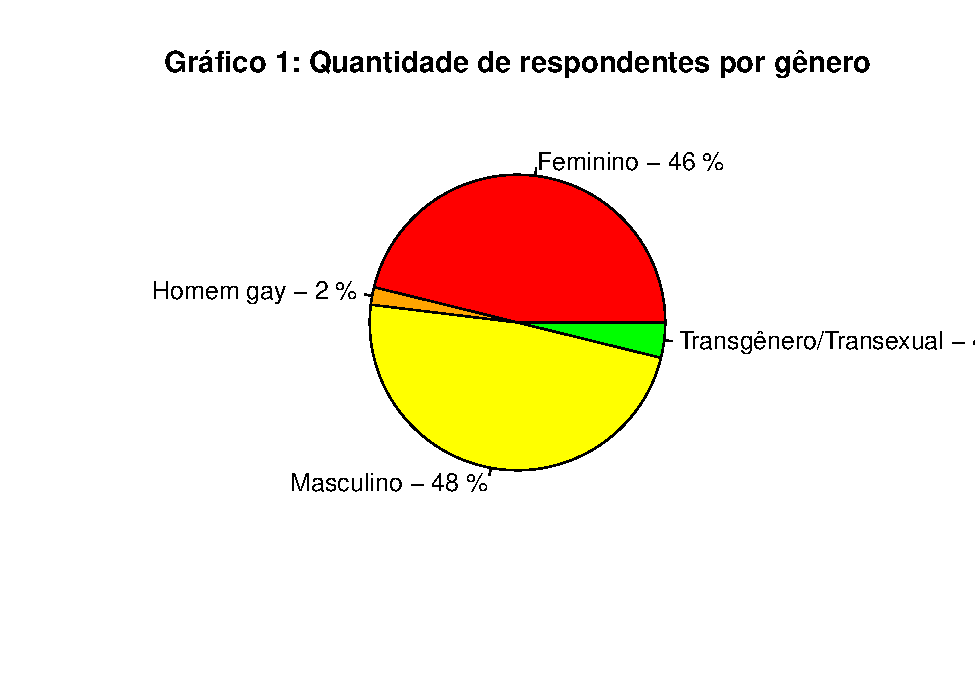
\includegraphics{consequencias-oriundas-da-pandemia-v1.0_files/figure-latex/grafico-1-1.pdf}

\hypertarget{anuxe1lise-exploratuxf3ria-de-dados}{%
\subsection{Análise Exploratória de
Dados}\label{anuxe1lise-exploratuxf3ria-de-dados}}

A Análise Exploratória de Dados (AED), de acordo com James et
al.~(2013), é uma abordagem de análise de dados que se concentra em
compreender e resumir as principais características dos dados por meio
de técnicas estatísticas e gráficas. O principal objetivo da AED é
descobrir padrões, tendências, anomalias e relações entre as variáveis
em um conjunto de dados, com o objetivo de gerar hipóteses e insights
para análises mais aprofundadas, afirmam os autores.\\
De acordo com Tukey (1977), o processo de AED envolve a ``coleta de
dados, organização, sumarização, análise exploratória, modelagem e
comunicação dos resultados''. A AED pode ser realizada tanto em
conjuntos de dados pequenos quanto grandes e complexos, e pode ser
aplicada em diversas áreas, como ciências sociais, biologia, economia,
engenharia, entre outras.

\hypertarget{perfil-dos-entrevistados}{%
\subsection{Perfil dos entrevistados}\label{perfil-dos-entrevistados}}

Para o perfil dos entrevistados foram analisadas as respostas obtidas
pelo questionário, no período disponível. A faixa etária com maior
número de entrevistados, correspondendo a 35\%, é a faixa etária de 17 a
24 anos. As faixas de 22 a 26 anos e 37 a 41 anos obtiveram 13\% cada
uma, 10\% dos respondentes estão na faixa de 42 a 46 anos, de 47 a 51
anos e de 52 a 56 anos tiveram ambas 8\%, 6\% eram da faixa de 27 a 31
anos, 6\% de 32 a 36 anos, e apenas 2\% se enquadraram na faixa etária
de 57 a 61 anos, como é possível observar no Gráfico 2.

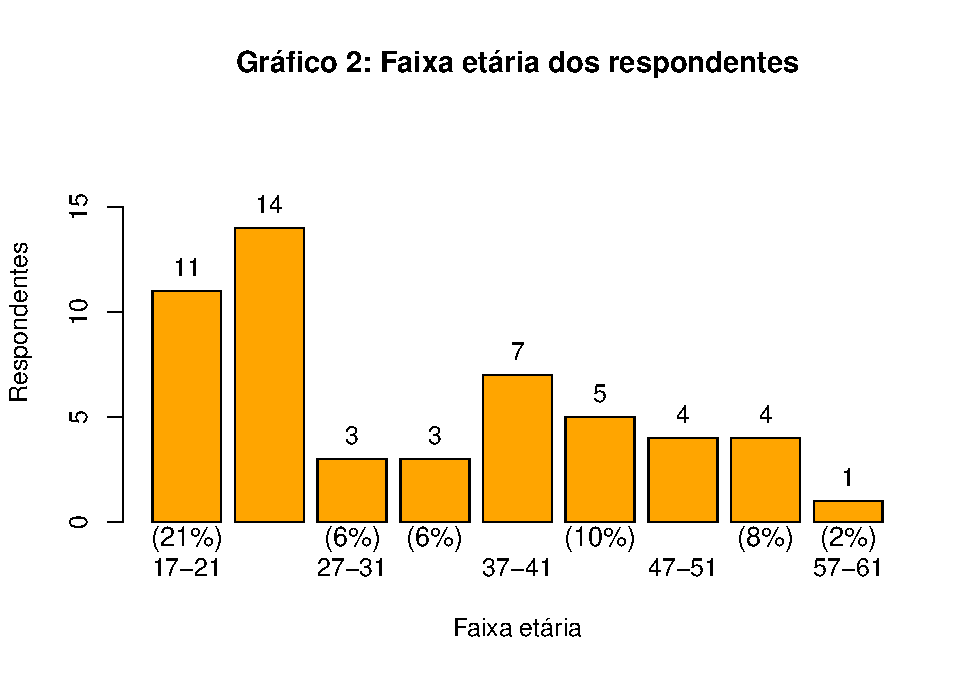
\includegraphics{consequencias-oriundas-da-pandemia-v1.0_files/figure-latex/grafico-2-1.pdf}

Quanto ao estado civil dos participantes 54\% são solteiros(as), 31\%
casados(as), 10\% estão em uma união estável, 4\% divorciados(as) e 1\%
viúvos(as). Tais dados estão representados no Gráfico 3

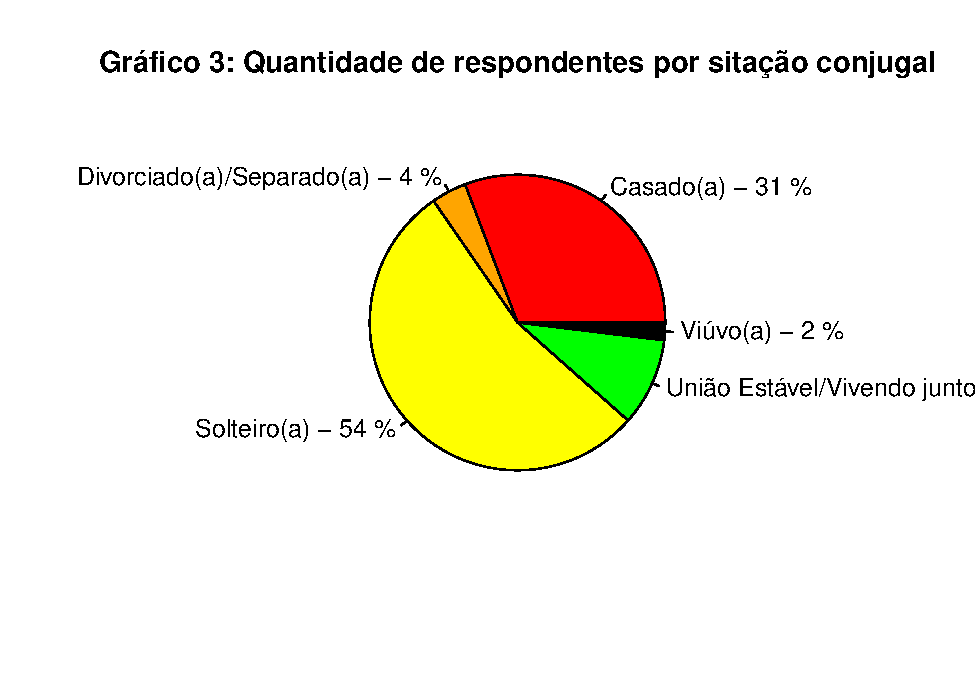
\includegraphics{consequencias-oriundas-da-pandemia-v1.0_files/figure-latex/grafico-3-1.pdf}

Ainda caracterizando o perfil dos entrevistados, na figura do Gráfico 4
foi apontado que o nível de escolaridade predominante da amostra é a
graduação, com 21 respondentes (40\%), seguido pelo doutorado com 15
(29\%) e mestrado com 13 respondentes.

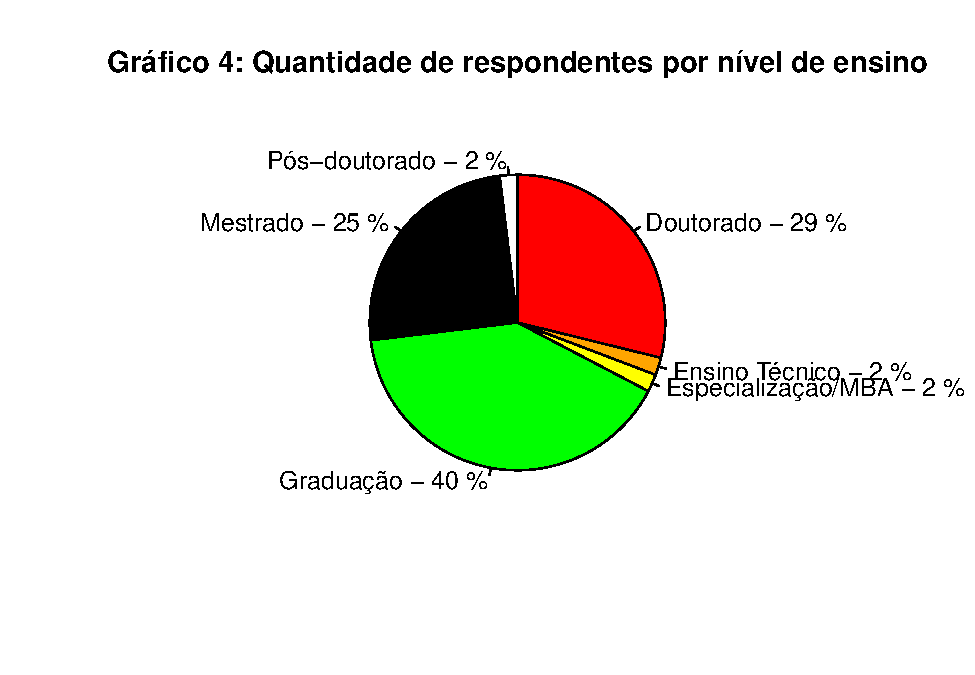
\includegraphics{consequencias-oriundas-da-pandemia-v1.0_files/figure-latex/grafico-4-1.pdf}

Observa-se no Gráfico 4 que os níveis de Pós-doutorado,
MBA/Especialização e ensino técnico constam 1 entrevistado cada (2\%).
Do total de respondentes da pesquisa, a grande maioria (86\%) são de
instituição pública, 12\% de instituições privadas, e 2\% de autarquia
municipal (Gráfico 5).

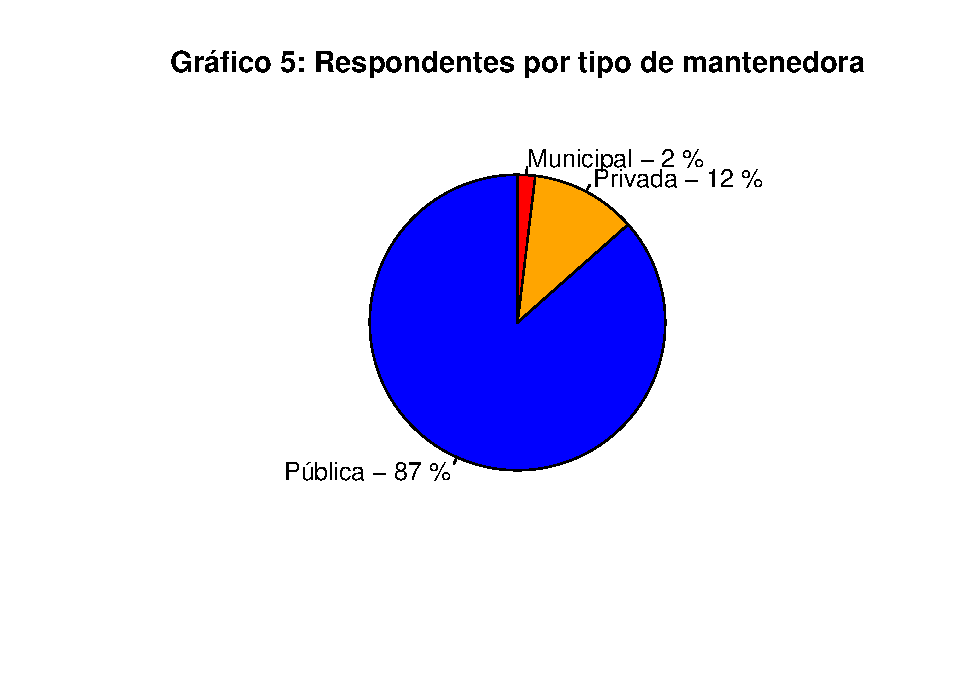
\includegraphics{consequencias-oriundas-da-pandemia-v1.0_files/figure-latex/grafico-5-1.pdf}

Ao analisar as condições financeiras dos participantes por meio do
Gráfico 6, foi possível identificar que, do total de participantes da
amostra, 56\% estavam empregados, em diversos segmentos, 23\% eram
bolsistas ou estagiários, 13\% eram dependentes e contavam com ajuda dos
pais, 2\% aposentados e 4\% estavam desempregados.

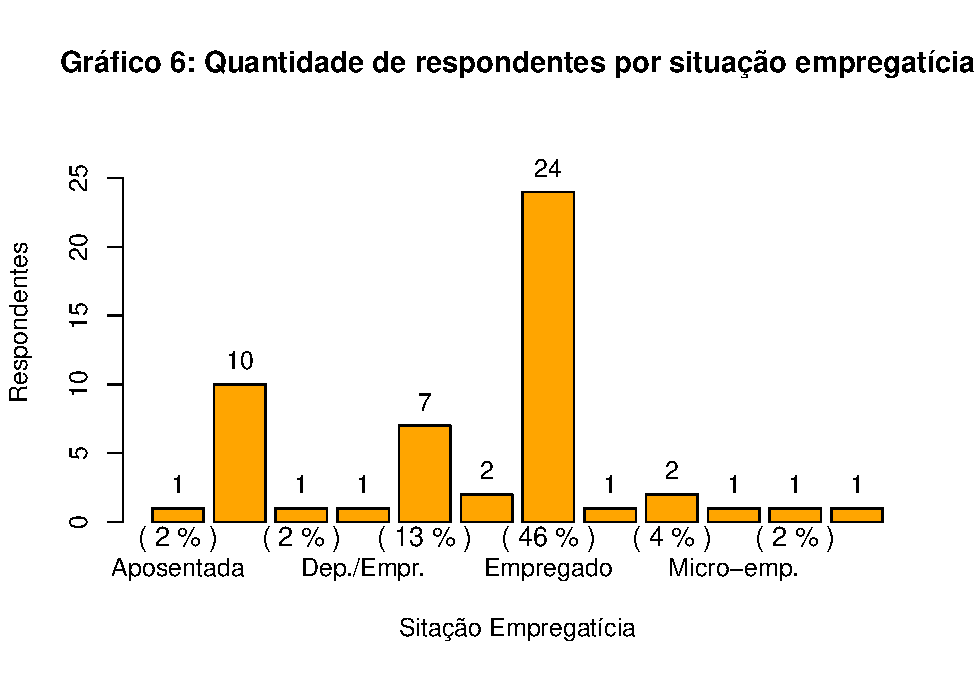
\includegraphics{consequencias-oriundas-da-pandemia-v1.0_files/figure-latex/grafico-6-1.pdf}

Com relação questão da vacinação, nesta amostra todos os participantes
foram vacinados contra a Covid-19, como é possível observar no Gráfico
8.

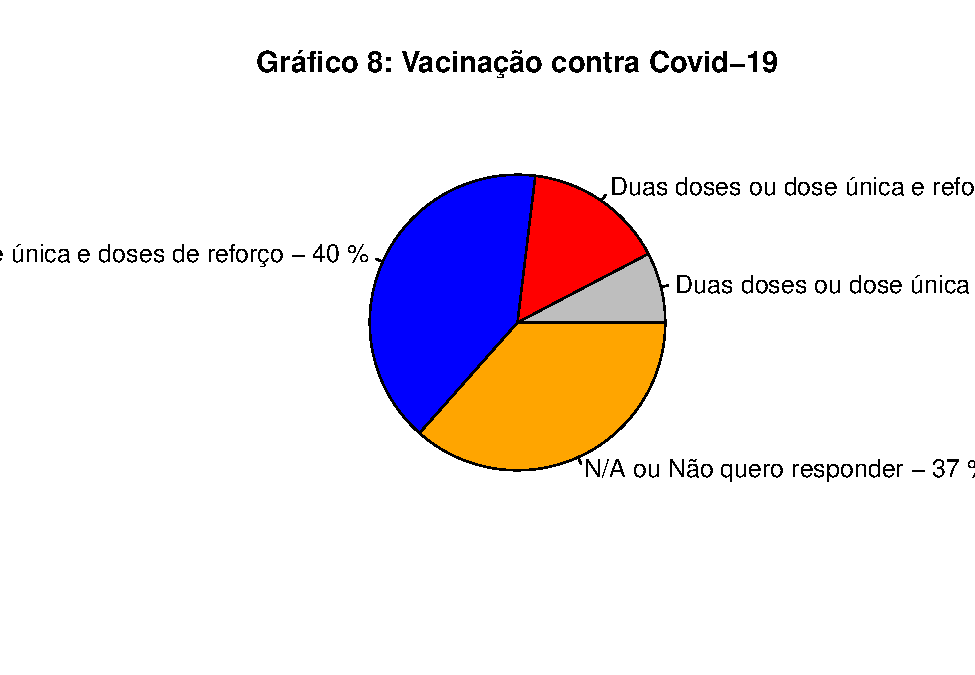
\includegraphics{consequencias-oriundas-da-pandemia-v1.0_files/figure-latex/grafico-8-1.pdf}

Em sua maioria, foram tomadas as duas doses, ou dose única além das
doses de reforço. Outro fator importante a ser levado em consideração
devido a pandemia é a questão de locomoção - impedidas pelas restrições
e \emph{lockdown} - e o fato de que a maior parte dos respondentes não
eram residentes da cidade em que estudavam, pois apenas 18 (35\%) dos
entrevistados eram residentes na mesma cidade da universidade e/ou
faculdade e a maioria, 34 (65\%) de outras cidades. Destes, 90\% estavam
na sua residência permanente durante a pandemia e 10\% não (Gráfico 9).

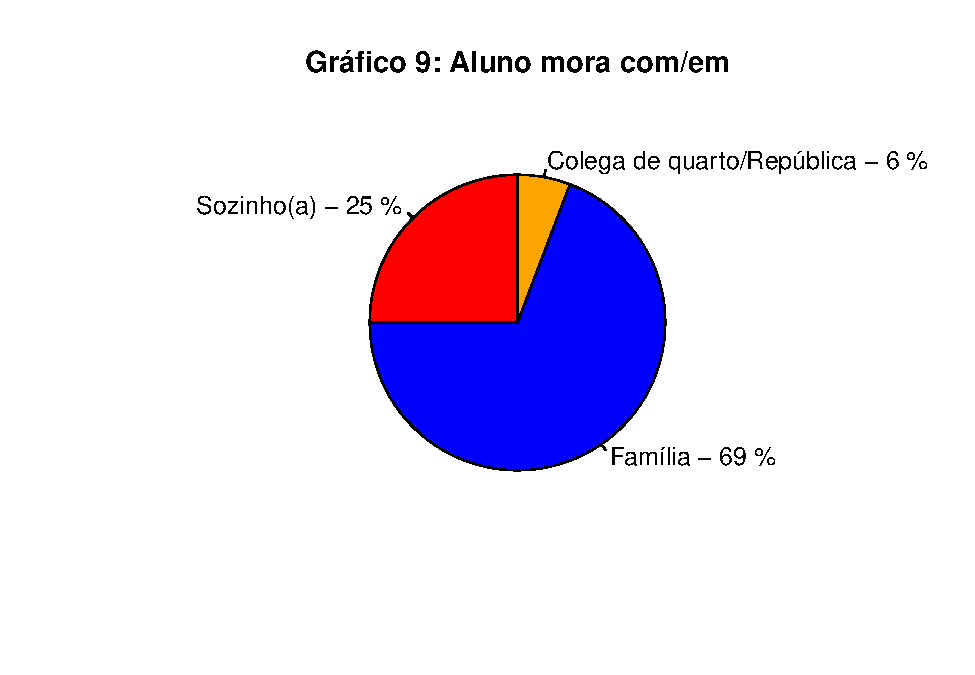
\includegraphics{consequencias-oriundas-da-pandemia-v1.0_files/figure-latex/grafico-9-1.pdf}

Conforme demonstrado no Gráfico 9, dos respondentes, 69\% moravam com a
família, seguido de 25\% morando sozinho e, em último ficaram os que
residiam em república ou com colega de quarto (6\%).

\hypertarget{decisuxf5es-tomadas-acesso-uxe0-infraestrutura-e-aos-docentes}{%
\subsection{Decisões tomadas, acesso à infraestrutura e aos
docentes}\label{decisuxf5es-tomadas-acesso-uxe0-infraestrutura-e-aos-docentes}}

Sobre a decisão de fechar o campus para evitar a circulação de pessoas
e, consequentemente, evitar a circulação do vírus, como pode ser
observado na figura do Gráfico 10, 77\% dos pesquisados consideram a
decisão tomada em momento oportuno, enquanto 13\% consideram lenta a
demora para a tomada de decisão e 10\% definem como muito rápido.

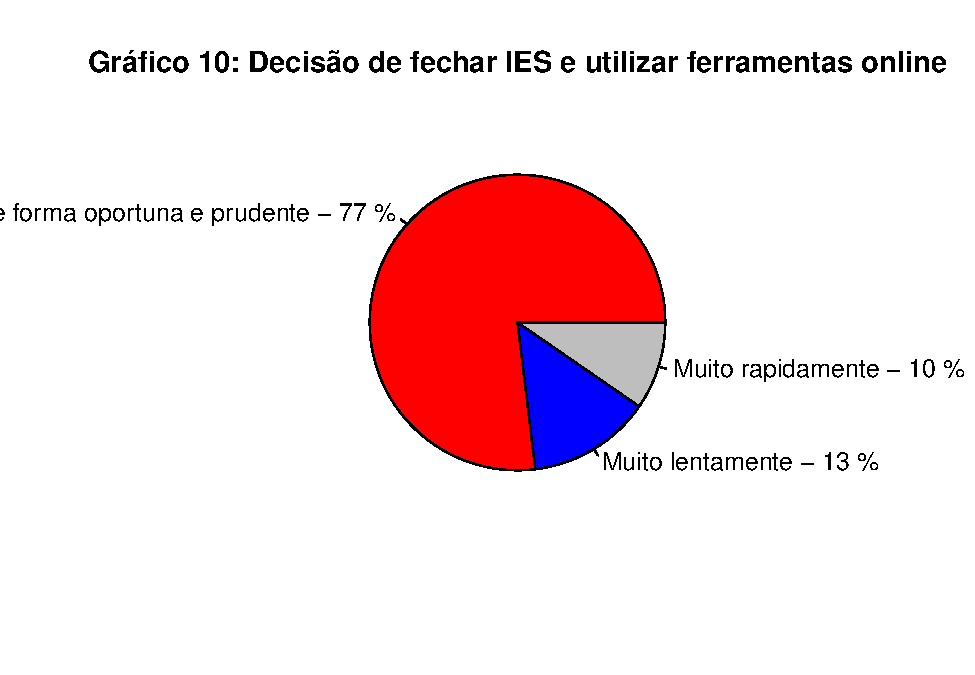
\includegraphics{consequencias-oriundas-da-pandemia-v1.0_files/figure-latex/grafico-10-1.pdf}

No que diz respeito à investigação se a Instituição de Nível Superior
(IES) durante a pandemia transferiu todas suas atividades presenciais
para o ensino remoto, apenas 2\% dos alunos da amostra informaram que
sua instituição não havia migrado para as aulas virtuais durante a
pandemia, entretanto, 98\% das IES da amostra se adaptaram de alguma
forma para educação remota, como mostra o Grafico 11.

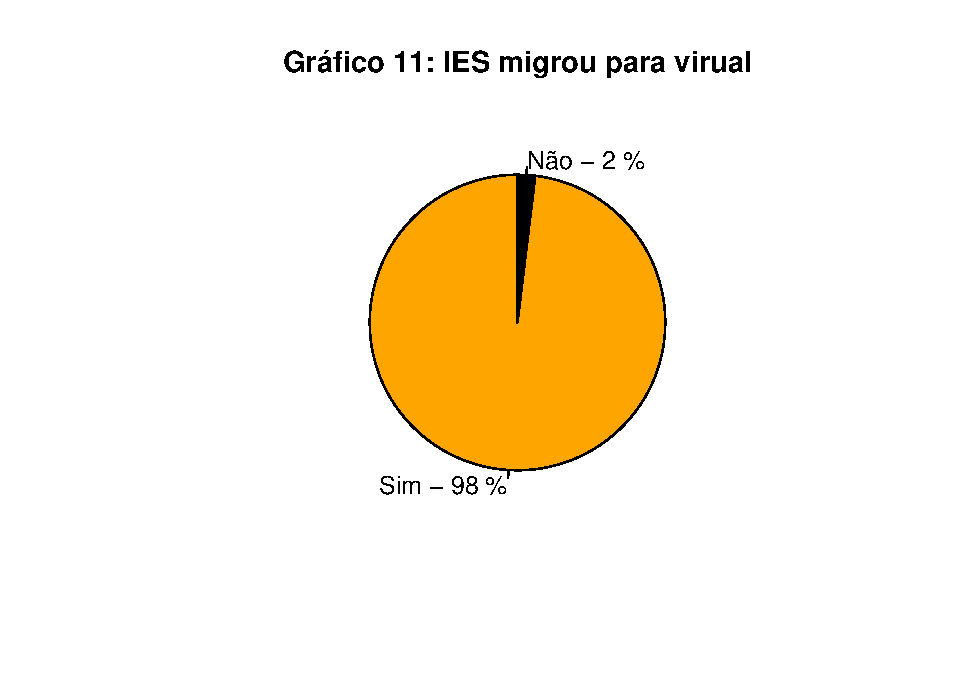
\includegraphics{consequencias-oriundas-da-pandemia-v1.0_files/figure-latex/grafico-11-1.pdf}

Já no tocante as formas de acesso aos recursos de infraestrutura
oferecidos pela instituição (biblioteca, coordenação, orientação de
assuntos acadêmicos, matrícula etc.) o Gráfico 12 mostra que, na opinião
de 40\% dos estudantes, o acesso aos recursos da IES pioraram durante a
pandemia do COVID-19. Já 33\% alegam que não houve mudanças.

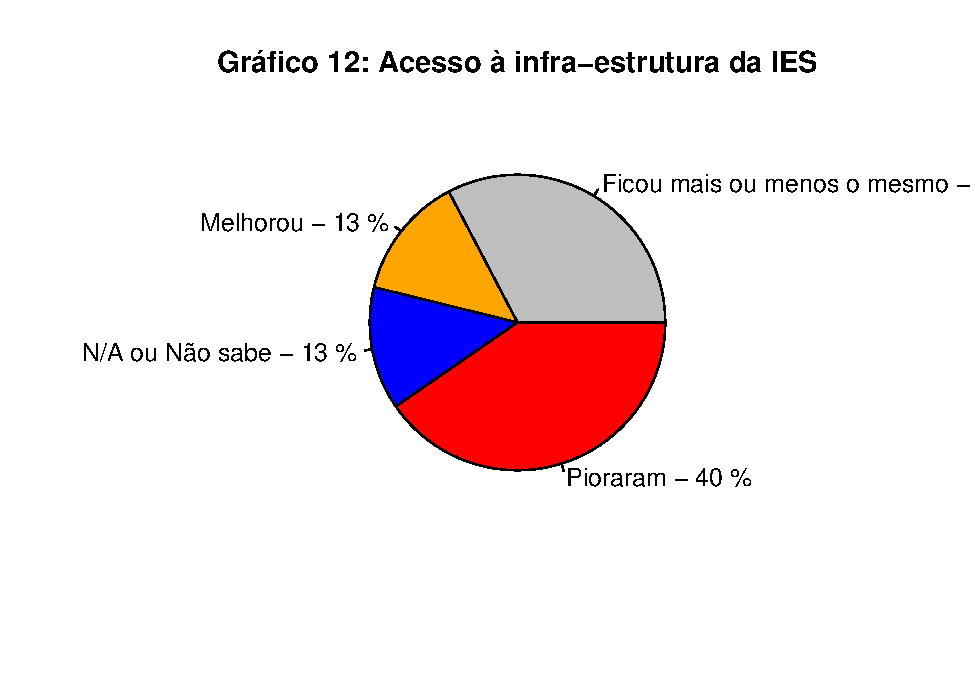
\includegraphics{consequencias-oriundas-da-pandemia-v1.0_files/figure-latex/grafico-12-1.pdf}

Os dados no Gráfico 12 indicam ainda que houve empate entre aqueles que
alegam que houve melhorias e os que não sabem responder, ambos os lados
representado 13\% da amostra.

Ao abordar o acesso ao corpo docente das IES durante a pandemia (Gráfico
13), a maioria dos respondentes sentiu que o acesso aos professores foi
pior (52\%) que antes da pandemia, seguido por aqueles que acharam que
não houve grandes dificuldades de comunicação (25\%). Para uma parcela
menor (15\%) a disponibilidade dos docentes melhorou e apenas 8\% não
souberam responder.

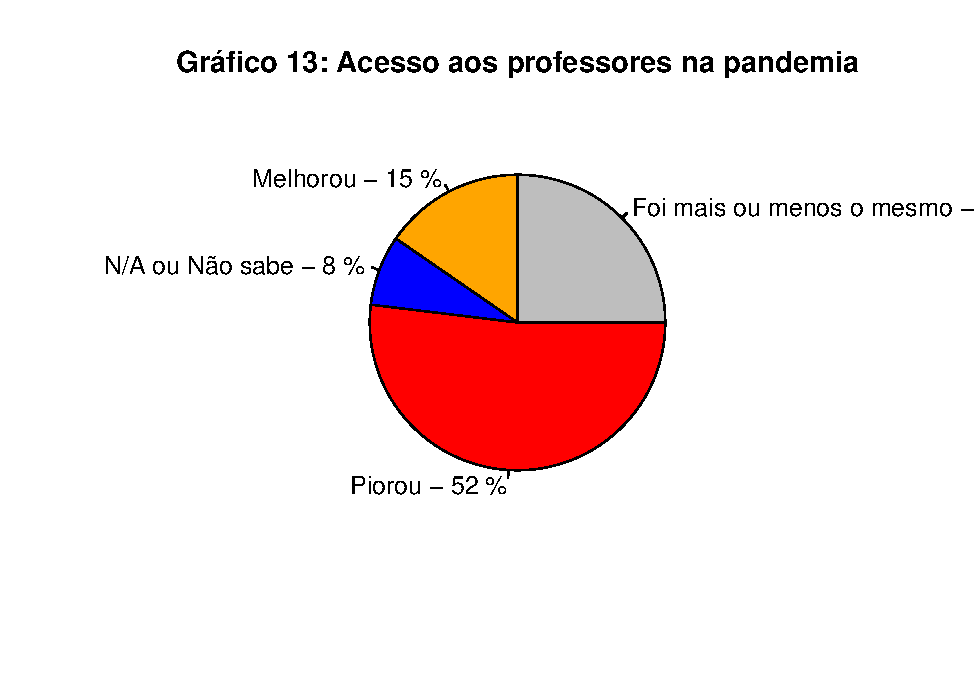
\includegraphics{consequencias-oriundas-da-pandemia-v1.0_files/figure-latex/grafico-13-1.pdf}

Quando questionados sobre a forma como as aulas foram ministradas
durante a pandemia, de acordo com figura do Gráfico 14, 48\% dos
participantes não sentiram nenhuma alteração. Entretanto, 42\% afirmaram
que as aulas ministradas no estilo remoto foram piores que pelo método
presencial, 8\% não souberam dizer e apenas 2\% acharam que o ensino
remoto foi melhor.

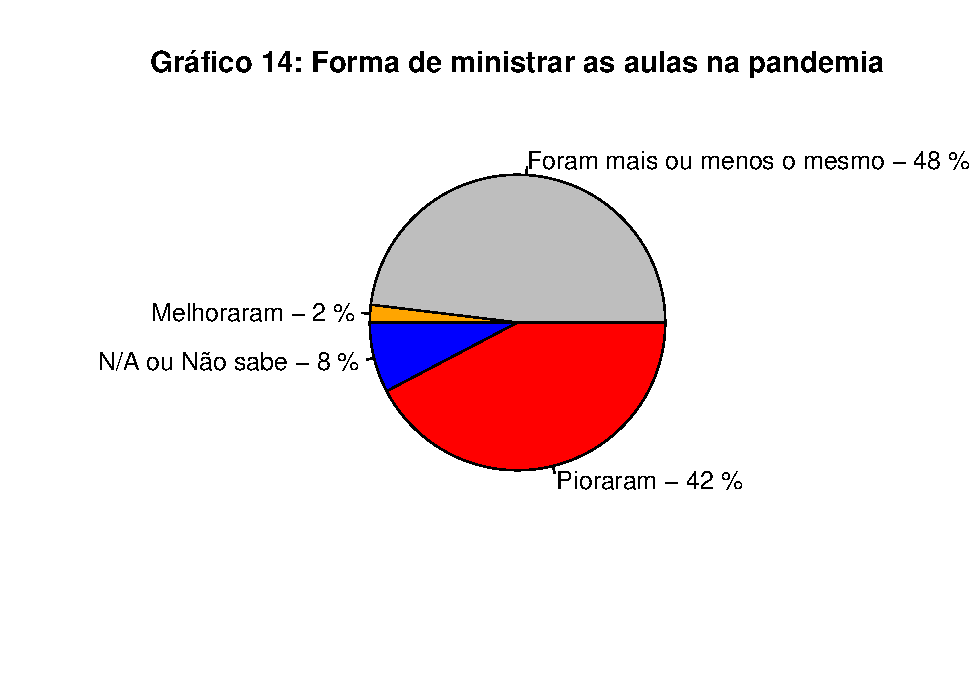
\includegraphics{consequencias-oriundas-da-pandemia-v1.0_files/figure-latex/grafico-14-1.pdf}

É interessante observar que, apesar de uma certa piora no acesso à
infraestrutura e professores, grande parte dos estudantes não se sentiu
afetado quanto à maneira como as aulas foram ministradas.\\
Após a vacinação e maior controle da pandemia, com dados coletados até o
final de 2022, 60\% dos entrevistados afirmaram que as universidades já
haviam retomado as atividades de forma presencial nas IES, 29\% haviam
retornado em parte, 8\% não haviam retomarado e 2\% não sabiam informar
(Gráfico 15).

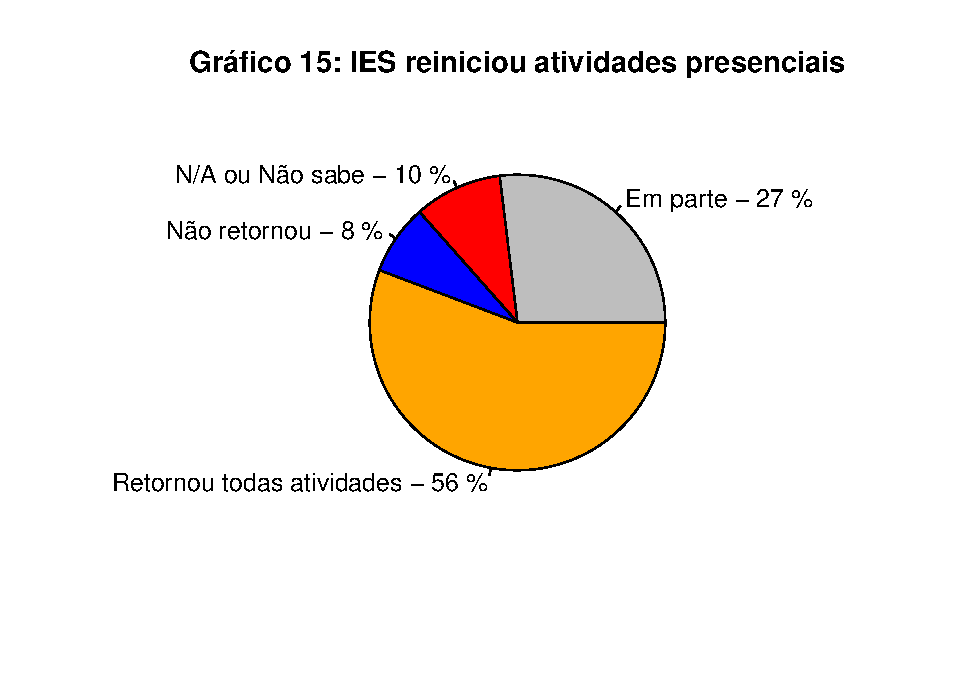
\includegraphics{consequencias-oriundas-da-pandemia-v1.0_files/figure-latex/grafico-15-1.pdf}

\hypertarget{dificuldades-enfrentadas-pelos-alunos}{%
\subsection{Dificuldades enfrentadas pelos
alunos}\label{dificuldades-enfrentadas-pelos-alunos}}

Buscando compreender as principais dificuldades individuais que os
alunos de ensino superior enfrentaram durante a pandemia, um conjunto de
questões foram elaboradas no questionário para coletar informações sobre
esforços que os estudantes tiveram que enfrentar para cursar as
disciplinas remotamente.\\
Partindo da necessidade em utilizar a internet para as aulas, os alunos
foram questionados quanto à qualidade do serviço de acesso à internet
que tiveram que utilizar, comparando a antes e durante a pandemia da
Covid-19.\\
De acordo com o Gráfico 16, 65\% dos respondentes afirmaram que não
houve nenhuma mudança, para 13\% o acesso aos serviços de internet
piorou e 19\% sentiram que houve melhora. Apenas 2\% não souberam
responder. De modo geral, para os estudantes pesquisados o acesso a
internet não mudou.

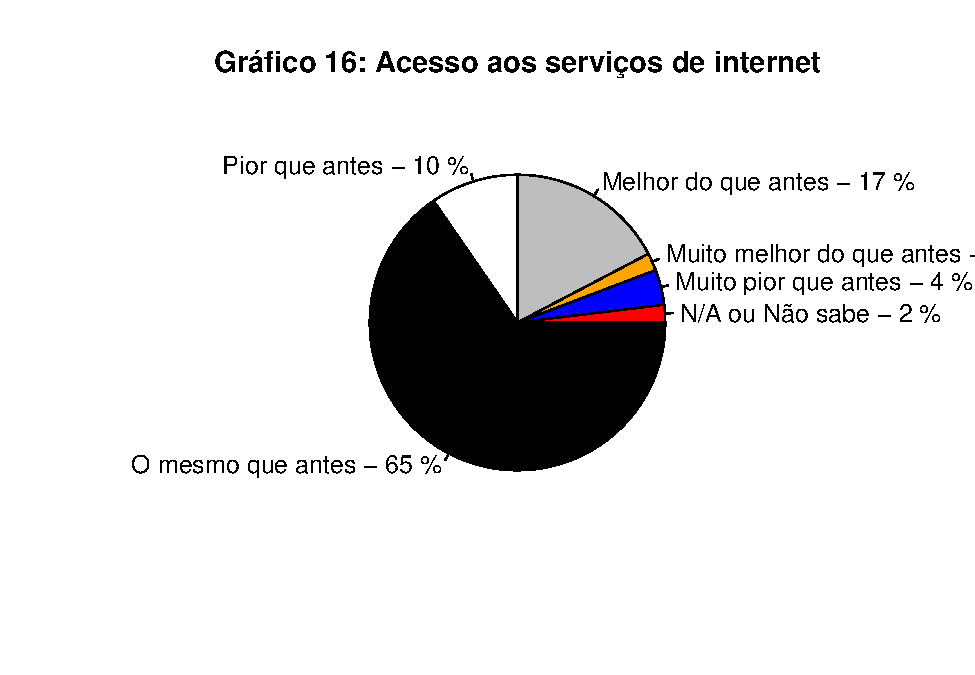
\includegraphics{consequencias-oriundas-da-pandemia-v1.0_files/figure-latex/grafico-16-1.pdf}

No que concerne à mudança para o ensino virtual remoto e a mudança na
forma de aprendizado, os dados do Gráfico 17 mostram que 38\% dos
participantes considera que não houve queda no seu desempenho escolar e
27\% consideram que o seu desempenho acadêmico aumentou no ensino
remoto, se comparado ao presencial.

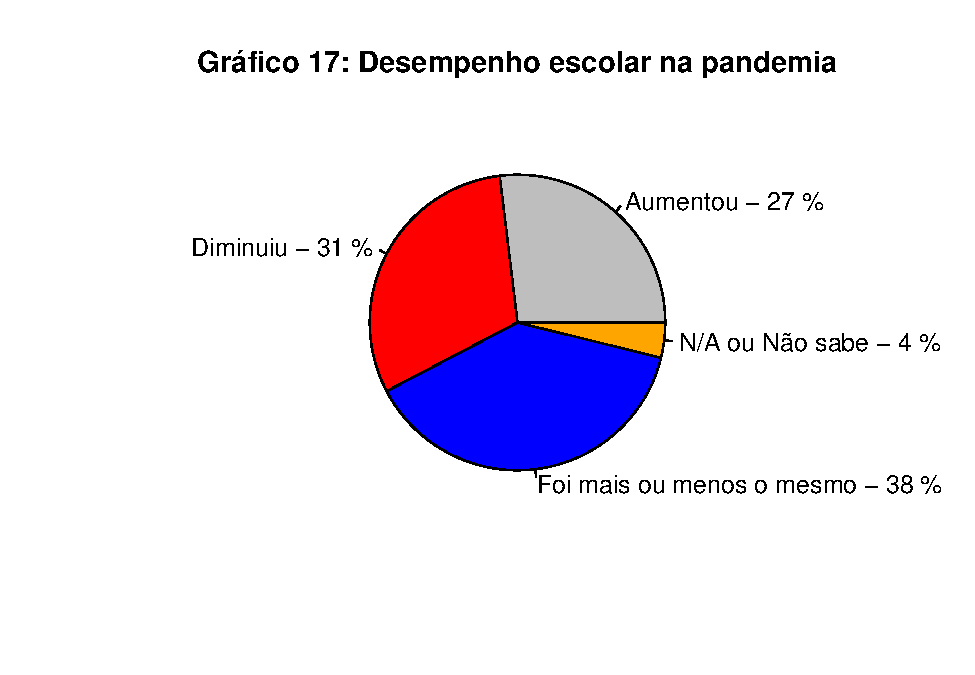
\includegraphics{consequencias-oriundas-da-pandemia-v1.0_files/figure-latex/grafico-30-1.pdf}

Entretanto, como também pode ser visualizado no Gráfico 17, 31\%
consideraram seu rendimento comprometido e 2\% não souberam opinar.\\
Com as restrições sociais introduzidas durante o período de isolamento
social, é importante também entender como a pandemia dificultou de forma
abrangente a vida dos docentes. Quando questionados diretamente quais os
fatos vivenciados durante o período agudo da pandemia que os afetaram
com intensidade, os alunos, de acordo com os dados do Gráfico 18,
responderam que, que pelas orientações de distanciamento e fechamento
dos serviços, tiveram dificuldades para se deslocar e/ou viajar (36\%),
além de necessitarem da ajuda de pessoas desconhecidas (8\%), sentiram
alguma discriminação por pessoas desconhecidas (2\%) e que tais
atribulações alteraram suas condições de vida (17\%) .

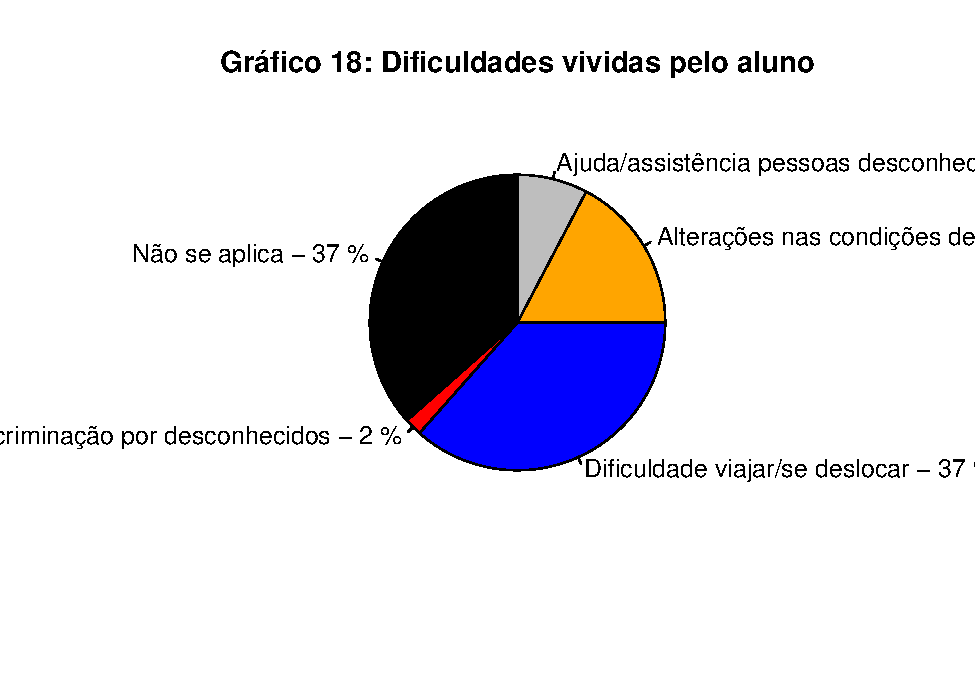
\includegraphics{consequencias-oriundas-da-pandemia-v1.0_files/figure-latex/grafico-18-1.pdf}

Além das dificuldades apontadas nos dados do Gráfico 18, dada as
restrições sociais a vida financeira dos discentes também foi afetada de
maneira importante. Os dados compilados no Gráfico 19 ilustram a
opiniãodos alunos em relação aos seus gastos durante o a pandemia onde
40\% alegam que as despesas não sofreram alteração, 33\% que houve
incremento nas suas despesas e 27\% tiveram redução.

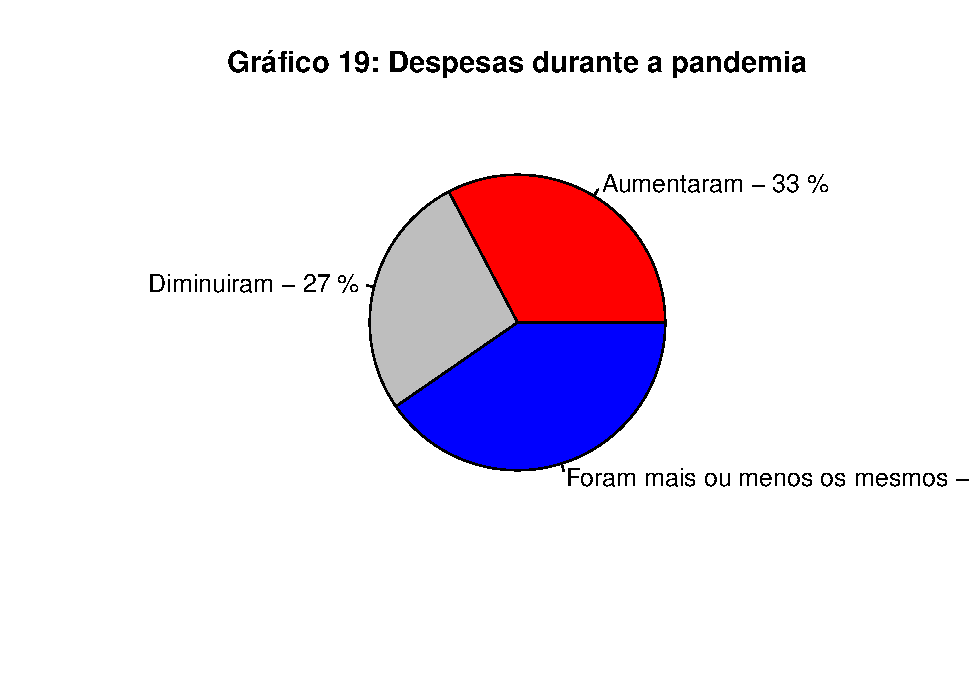
\includegraphics{consequencias-oriundas-da-pandemia-v1.0_files/figure-latex/grafico-34-1.pdf}

Apesar da maioria dos entrevistados não terem sofrido com o aumento de
despesas, já com relação ao seu poder de compra observamos no Gráfico 20
que 48\% observaram uma queda no seu poder de compra e 44\% consideram
que sua renda continuou mais ou menos a mesma.

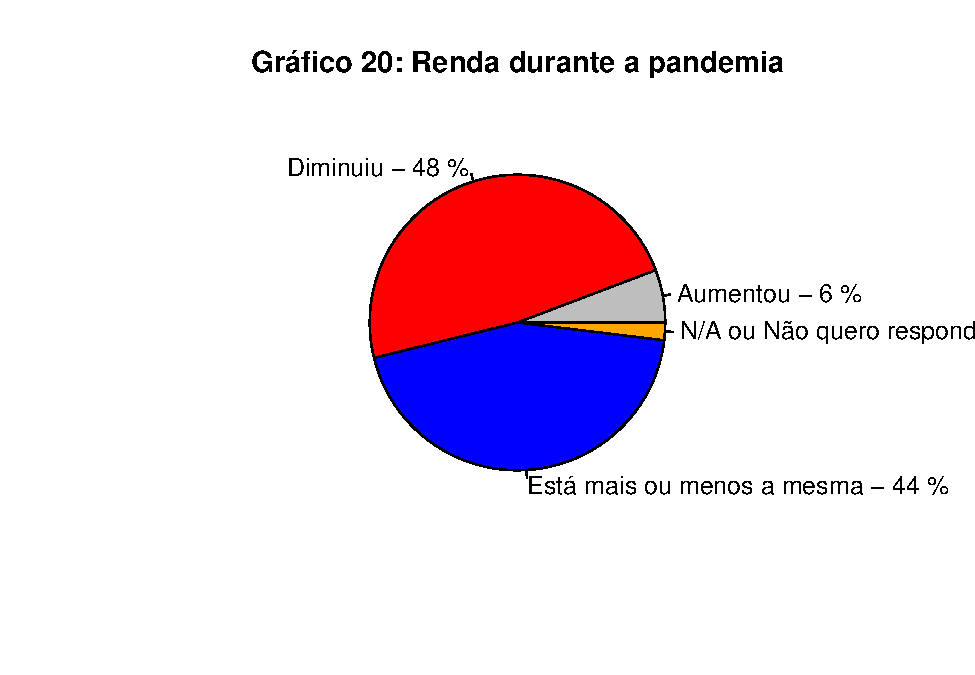
\includegraphics{consequencias-oriundas-da-pandemia-v1.0_files/figure-latex/grafico-20-1.pdf}

Como pode ser observado no Gráfico 20, apenas 6\% tiveram aumento nos
rendimentos e 2\% não quiseram e/ou souberam opinar.

Ainda que muitas universidades públicas ofereçam auxílio financeiro para
que estudantes possam morar no campus (ou próximo de) para estudarem, de
acordo com os dados do Gráfico 21 observa-se que durante o período de
pandemia 85\% dos entrevistados não tiveram nenhum respaldo por parte da
instituição educacional ou de outra organização.

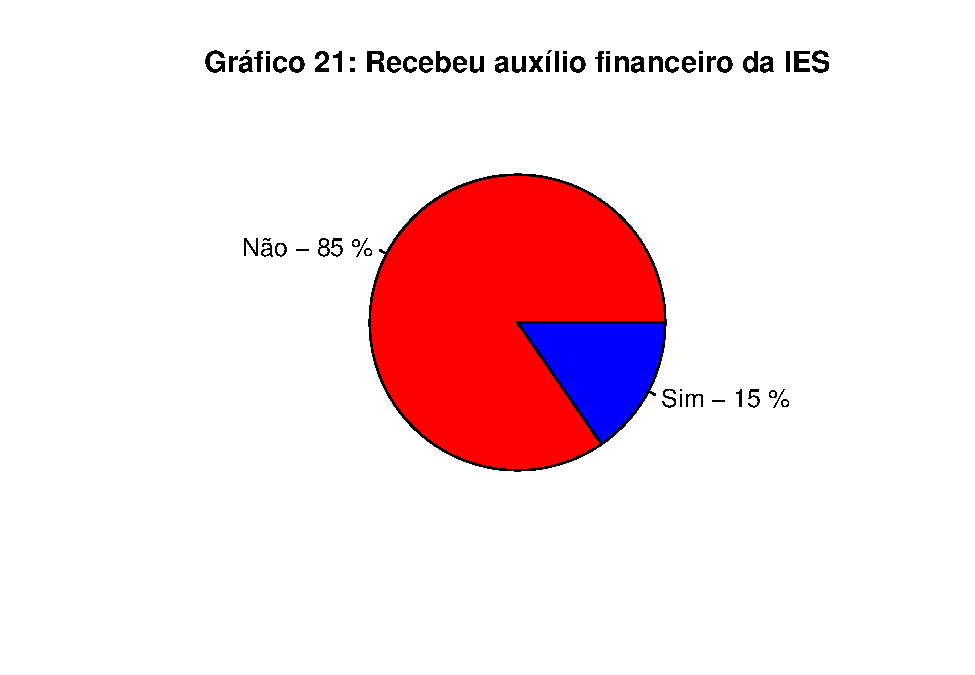
\includegraphics{consequencias-oriundas-da-pandemia-v1.0_files/figure-latex/grafico-21-1.pdf}

Quanto ao nível de endividamento durante a pandemia, os estudantes
afirmaram que 69\% não tiveram alteração nos seus débitos, como é
possível observar no Gráfico 22.

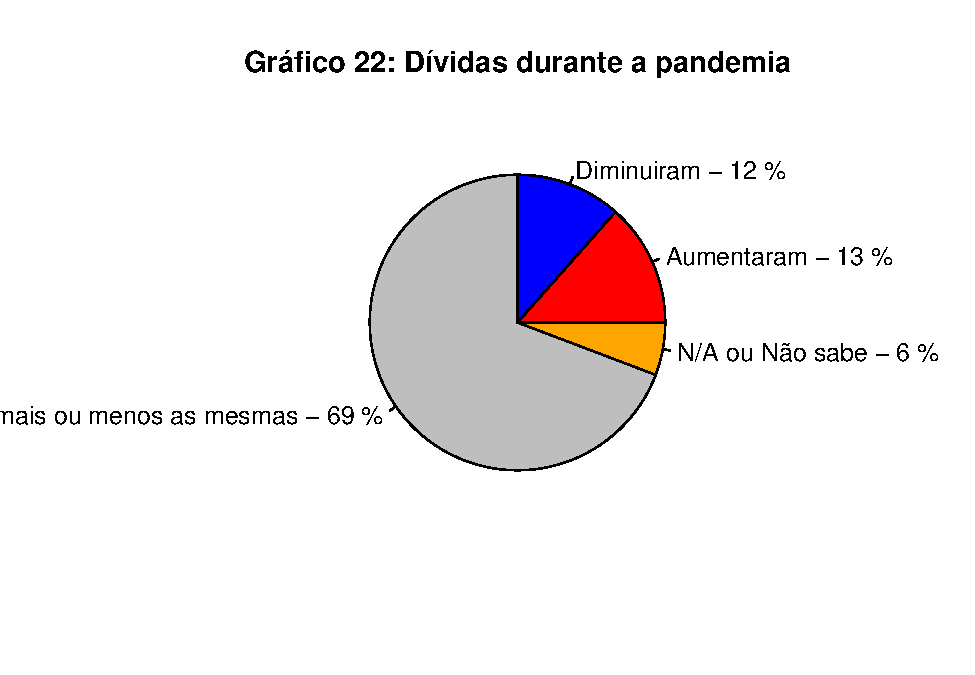
\includegraphics{consequencias-oriundas-da-pandemia-v1.0_files/figure-latex/grafico-22-1.pdf}

Já 13\% afirmaram ter aumentado o seu nível de endividamento, 12\% uma
diminuição, e 6\% não souberam informar, como ilustram os dados no
Gráfico 22. Pensando em um cenário ``pós-pandêmico'' (após o pico da
pandemia 2020/2022), foi solicitado aos participantes manifestar quais
gastos realizados por cada estudante que cresceram em diversos
segmentos. Nesta questão de resposta múltipla os respondentes poderiam
indicar mais de um segmento concomitantemente. Os dados compilados das
respostas estão ilustrados no Gráfico 23.

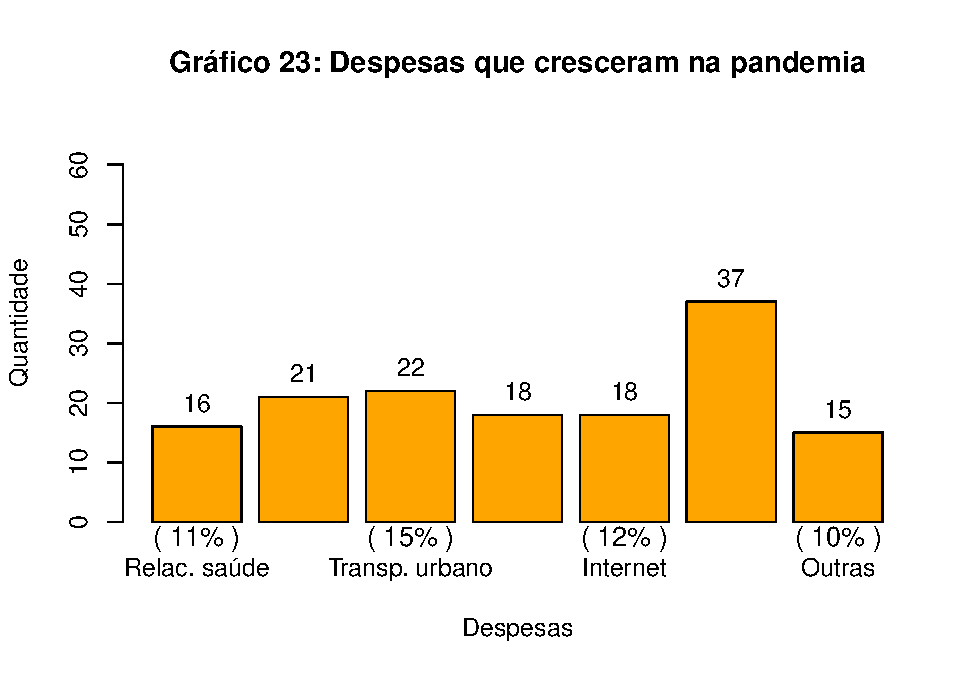
\includegraphics{consequencias-oriundas-da-pandemia-v1.0_files/figure-latex/grafico-23-1.pdf}

Dentre os gastos citados pelos respondentes pós pandemia e agrupados na
figura do Gráfico 22, observa-se que o maior crescimento apontado foi
com alimentação (25\%), seguido pelo transporte urbano (15\%) e
deslocamento (14\%). Levando em consideração que, em sua maioria, os
entrevistados tiveram que retomar pelo menos parcialmente ou de forma
híbrida para seu trabalho e faculdade, tais despesas justificam ser os
itens mais sinalizados.

\hypertarget{anuxe1lise-qualitativa}{%
\subsection{Análise qualitativa}\label{anuxe1lise-qualitativa}}

Questões com gráfico de chuvas de palavras! Como agregar e analisá-las ?

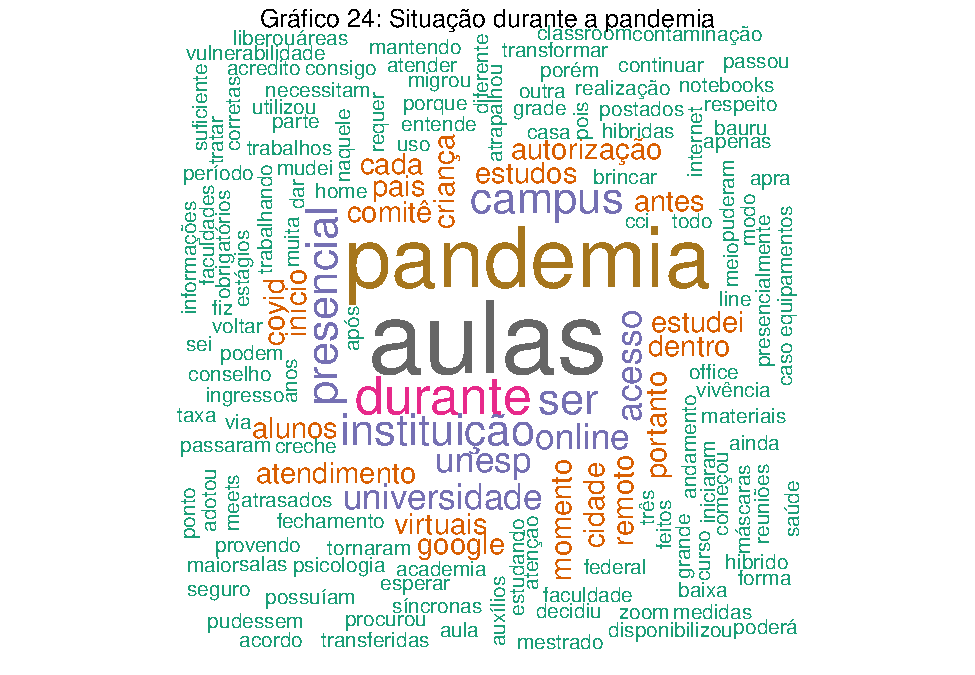
\includegraphics{consequencias-oriundas-da-pandemia-v1.0_files/figure-latex/grafico-24-1.pdf}

\begin{verbatim}
## [1] "Principais ocorrências de palavras em situação durante a pandemia"
\end{verbatim}

\begin{verbatim}
## [1] "aulas = 11"
## [1] "pandemia = 9"
## [1] "durante = 5"
## [1] "instituição = 4"
## [1] "ser = 4"
## [1] "presencial = 4"
## [1] "campus = 4"
## [1] "unesp = 3"
## [1] "online = 3"
## [1] "universidade = 3"
## [1] "acesso = 3"
\end{verbatim}

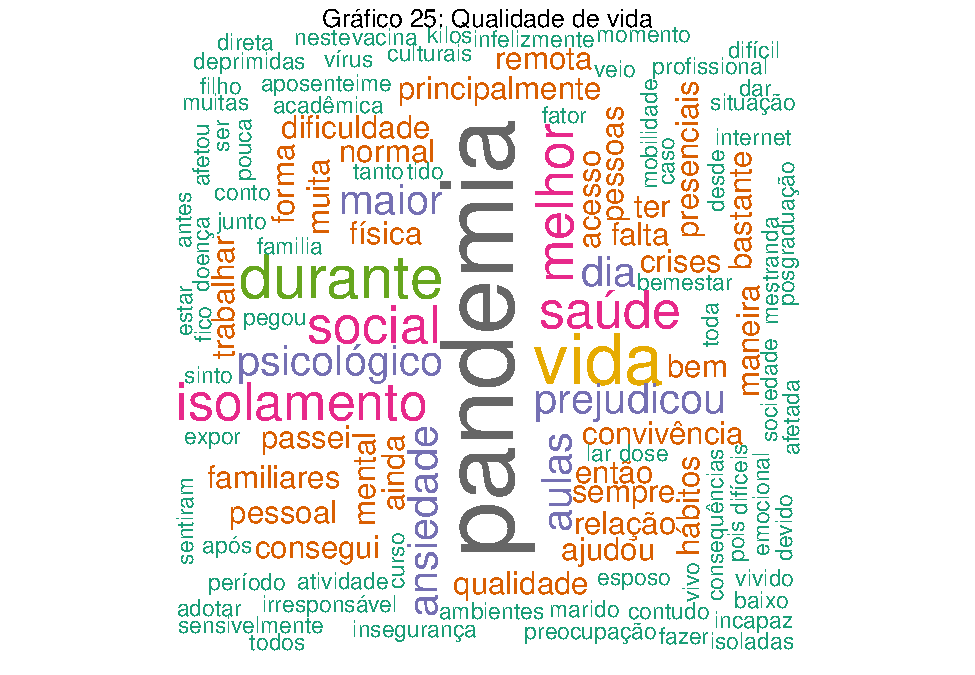
\includegraphics{consequencias-oriundas-da-pandemia-v1.0_files/figure-latex/grafico-25-1.pdf}

\begin{verbatim}
## [1] "Principais ocorrências de palavras em qualidade de vida"
\end{verbatim}

\begin{verbatim}
## [1] "pandemia = 9"
## [1] "vida = 6"
## [1] "durante = 5"
## [1] "saúde = 4"
## [1] "social = 4"
## [1] "isolamento = 4"
## [1] "melhor = 4"
## [1] "prejudicou = 3"
## [1] "psicológico = 3"
## [1] "ansiedade = 3"
## [1] "aulas = 3"
## [1] "dia = 3"
## [1] "maior = 3"
\end{verbatim}

\hypertarget{section}{%
\subsubsection{-----------------------------------------------------------}\label{section}}

\hypertarget{gruxe1ficos-opinando-com-relauxe7uxe3o-uxe0s-auxe7uxf5es-tomadas-pela-ies}{%
\subsubsection{Gráficos opinando com relação às ações tomadas pela
IES}\label{gruxe1ficos-opinando-com-relauxe7uxe3o-uxe0s-auxe7uxf5es-tomadas-pela-ies}}

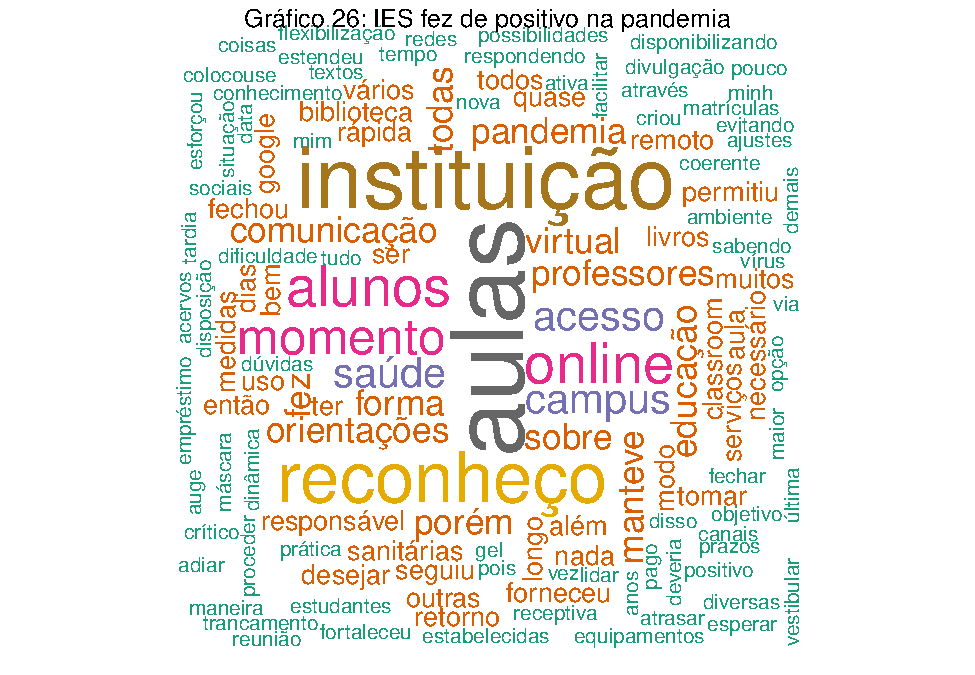
\includegraphics{consequencias-oriundas-da-pandemia-v1.0_files/figure-latex/grafico-26-1.pdf}

\begin{verbatim}
## [1] "Principais ocorrências de palavras do que a IES fez de positivo na pandemia"
\end{verbatim}

\begin{verbatim}
## [1] "aulas = 12"
## [1] "instituição = 10"
## [1] "reconheço = 8"
## [1] "alunos = 6"
## [1] "online = 6"
## [1] "momento = 5"
## [1] "acesso = 4"
## [1] "saúde = 4"
## [1] "campus = 4"
## [1] "forma = 3"
## [1] "professores = 3"
## [1] "virtual = 3"
## [1] "orientações = 3"
## [1] "comunicação = 3"
## [1] "manteve = 3"
## [1] "sobre = 3"
## [1] "porém = 3"
## [1] "pandemia = 3"
## [1] "fez = 3"
## [1] "educação = 3"
## [1] "todas = 3"
\end{verbatim}

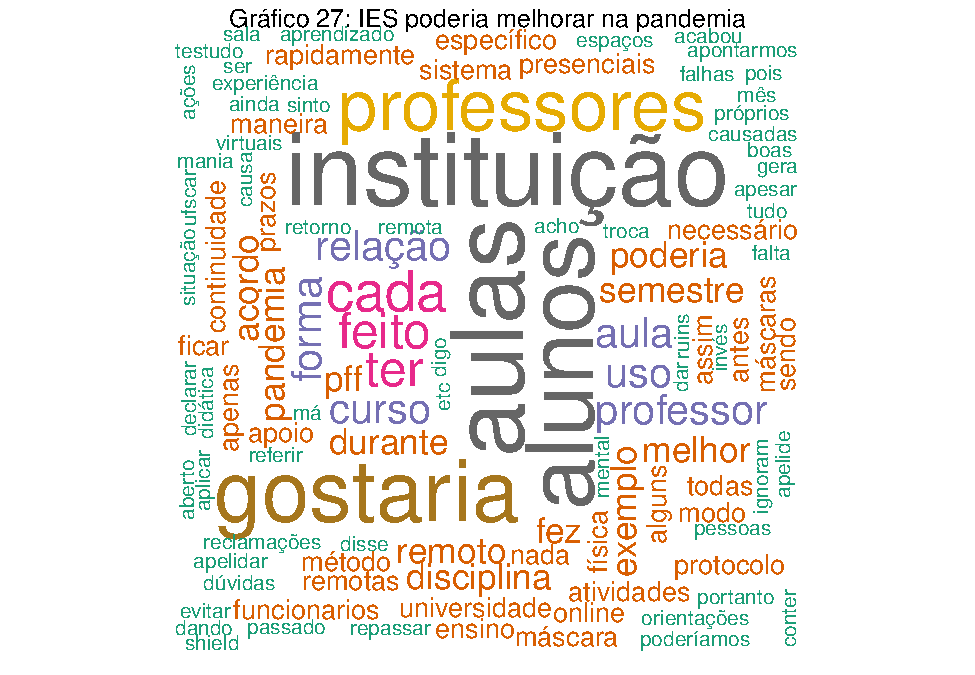
\includegraphics{consequencias-oriundas-da-pandemia-v1.0_files/figure-latex/grafico-27-1.pdf}

\begin{verbatim}
## [1] "Principais ocorrências de palavras do que a IES poderia melhorar na pandemia"
\end{verbatim}

\begin{verbatim}
## [1] "aulas = 12"
## [1] "instituição = 12"
## [1] "alunos = 11"
## [1] "gostaria = 10"
## [1] "professores = 8"
## [1] "cada = 6"
## [1] "feito = 5"
## [1] "ter = 5"
## [1] "relação = 4"
## [1] "curso = 4"
## [1] "professor = 4"
## [1] "uso = 4"
## [1] "aula = 4"
## [1] "forma = 4"
## [1] "durante = 3"
## [1] "exemplo = 3"
## [1] "pandemia = 3"
## [1] "semestre = 3"
## [1] "poderia = 3"
## [1] "remoto = 3"
## [1] "acordo = 3"
## [1] "melhor = 3"
## [1] "disciplina = 3"
## [1] "fez = 3"
## [1] "pff = 3"
\end{verbatim}

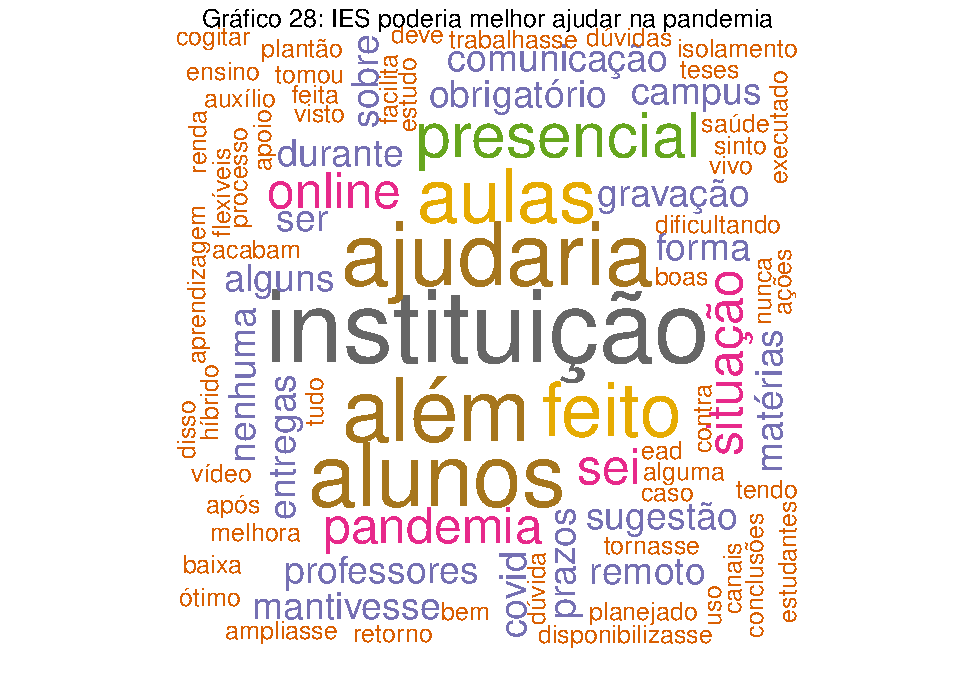
\includegraphics{consequencias-oriundas-da-pandemia-v1.0_files/figure-latex/grafico-28-1.pdf}

\begin{verbatim}
## [1] "Principais ocorrências de palavras do que a IES poderia melhora ajudar na pandemia"
\end{verbatim}

\begin{verbatim}
## [1] "instituição = 7"
## [1] "ajudaria = 6"
## [1] "além = 6"
## [1] "alunos = 6"
## [1] "aulas = 5"
## [1] "feito = 5"
## [1] "presencial = 4"
## [1] "pandemia = 3"
## [1] "sei = 3"
## [1] "online = 3"
## [1] "situação = 3"
\end{verbatim}

\hypertarget{section-1}{%
\subsection{------------------------------------------------------}\label{section-1}}

\hypertarget{gruxe1ficos-avaliando-a-situauxe7uxe3o-psicoluxf3gica-dos-alunos}{%
\subsection{Gráficos avaliando a situação psicológica dos
alunos}\label{gruxe1ficos-avaliando-a-situauxe7uxe3o-psicoluxf3gica-dos-alunos}}

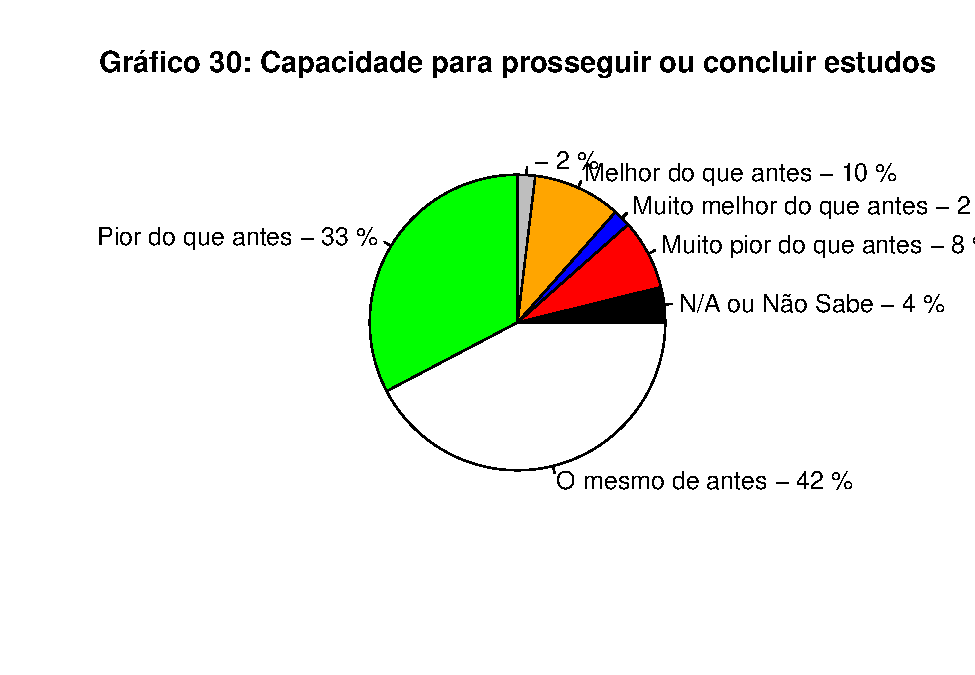
\includegraphics{consequencias-oriundas-da-pandemia-v1.0_files/figure-latex/grafico-nono-1.pdf}

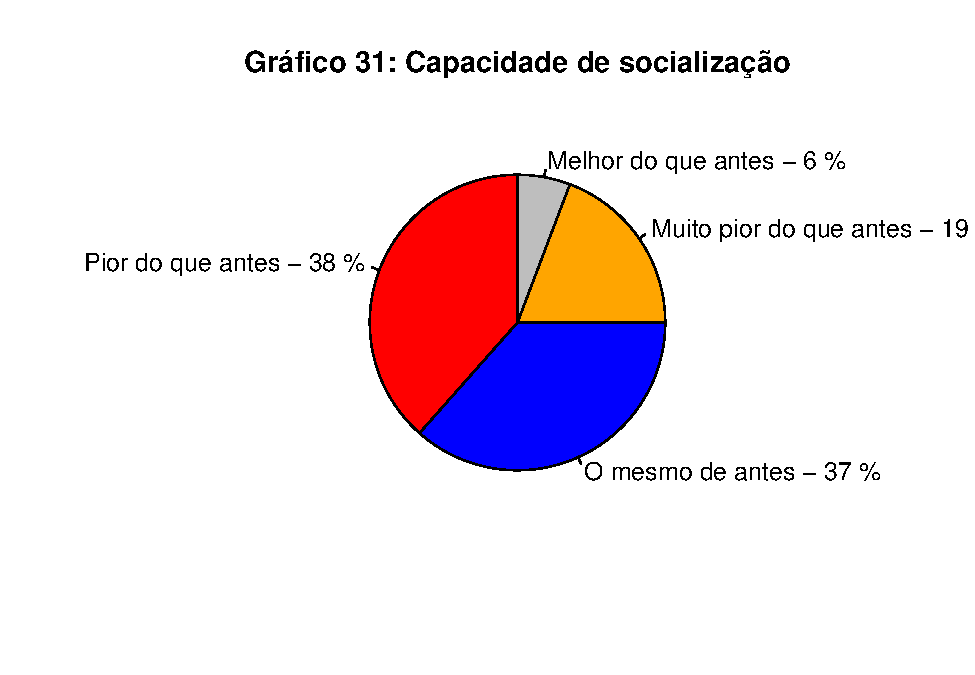
\includegraphics{consequencias-oriundas-da-pandemia-v1.0_files/figure-latex/grafico-xoxo-1.pdf}

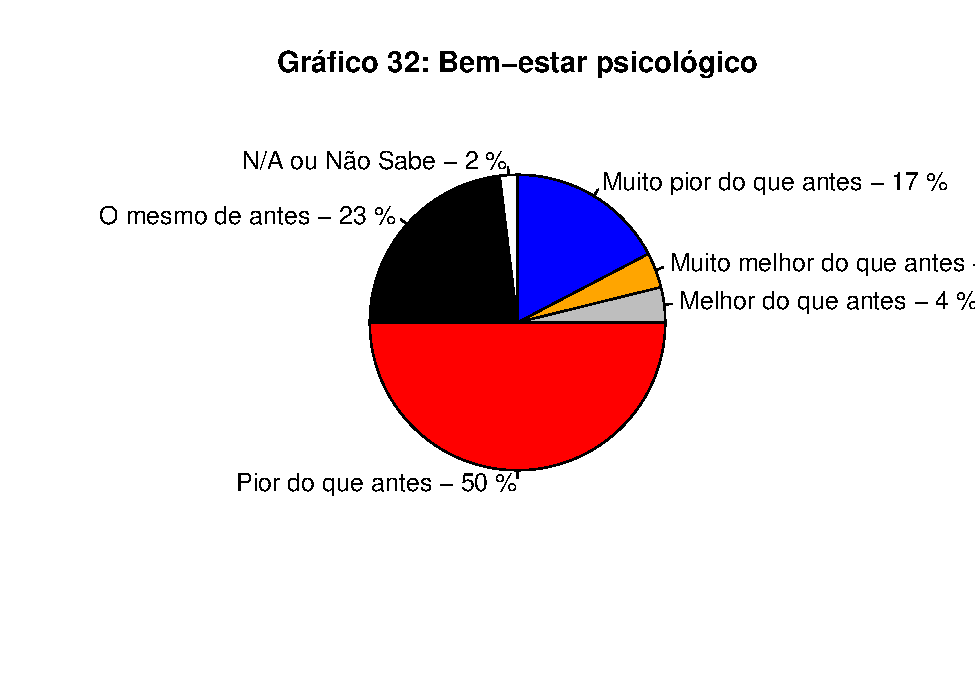
\includegraphics{consequencias-oriundas-da-pandemia-v1.0_files/figure-latex/grafico-yoyo-1.pdf}

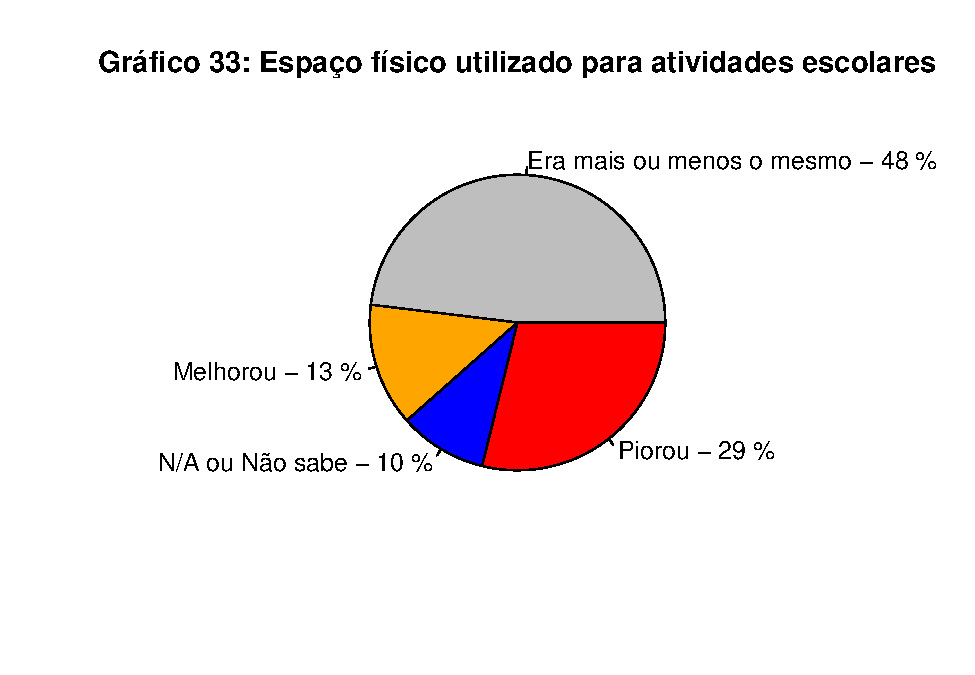
\includegraphics{consequencias-oriundas-da-pandemia-v1.0_files/figure-latex/grafico-zaza-1.pdf}

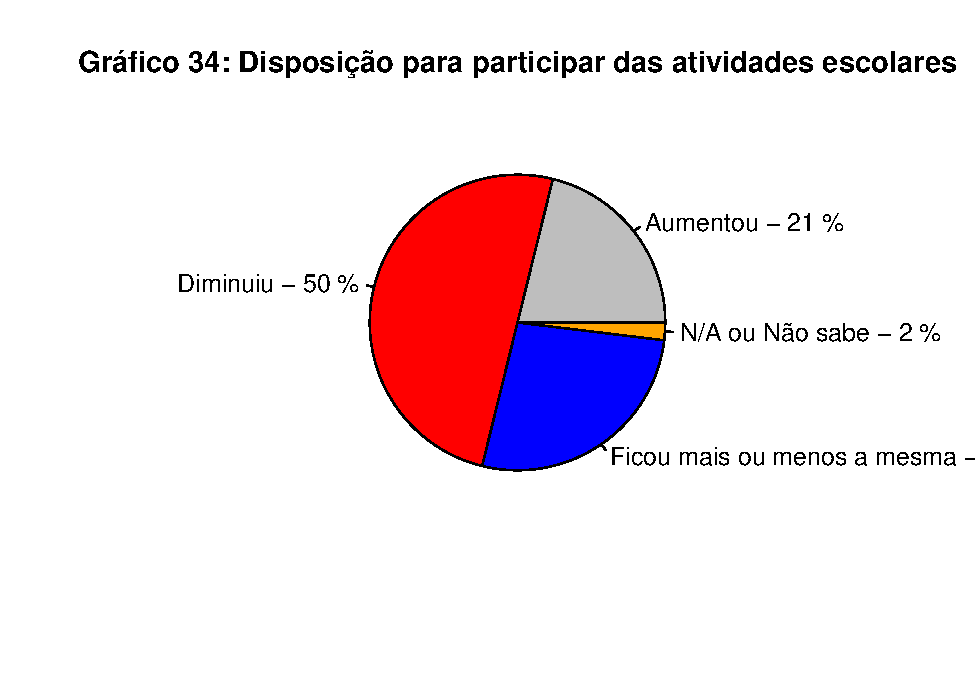
\includegraphics{consequencias-oriundas-da-pandemia-v1.0_files/figure-latex/grafico-mana-1.pdf}

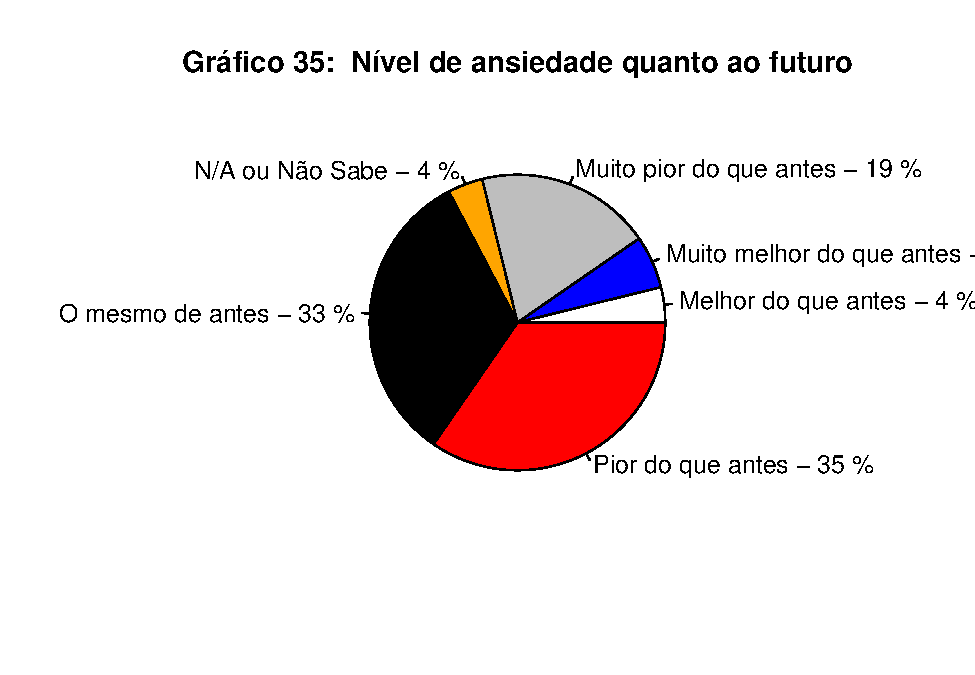
\includegraphics{consequencias-oriundas-da-pandemia-v1.0_files/figure-latex/grafico-mona-1.pdf}

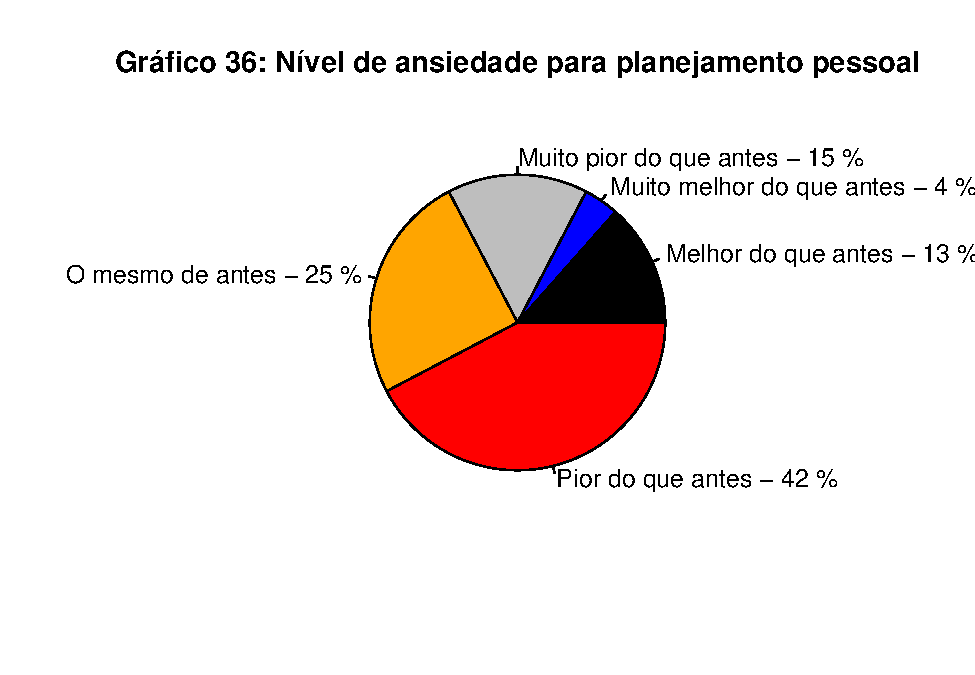
\includegraphics{consequencias-oriundas-da-pandemia-v1.0_files/figure-latex/grafico-zumba-1.pdf}

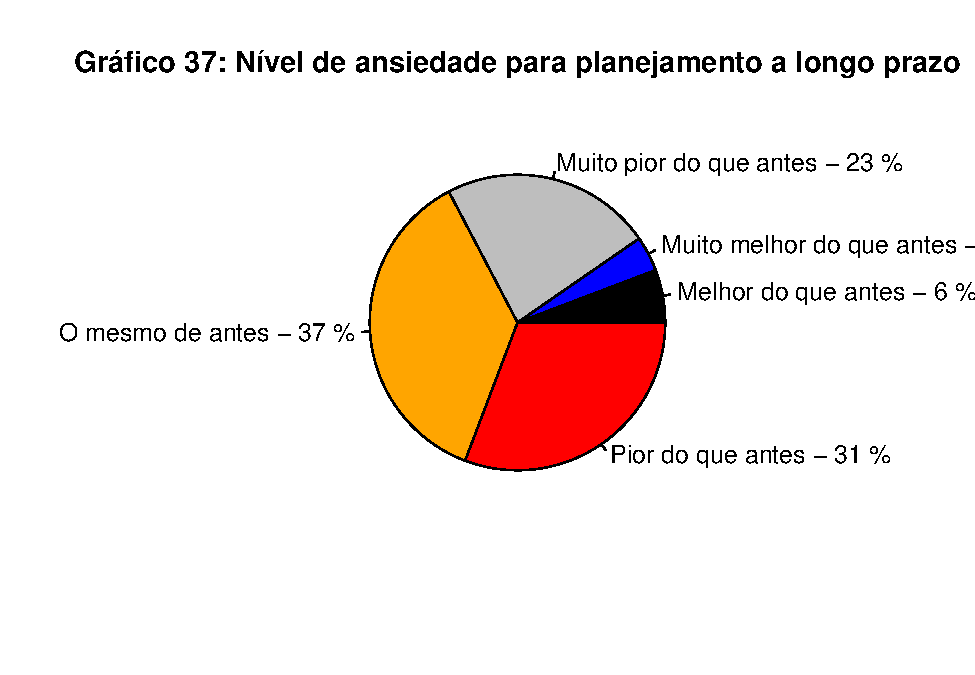
\includegraphics{consequencias-oriundas-da-pandemia-v1.0_files/figure-latex/grafico-cuca-1.pdf}

\hypertarget{section-2}{%
\subsection{--------------------------------------------------}\label{section-2}}

\hypertarget{opiniuxe3o-dos-alunos-sobre-as-dificuldades---principais-palavras-utilizadas}{%
\subsection{Opinião dos alunos sobre as dificuldades - principais
palavras
utilizadas}\label{opiniuxe3o-dos-alunos-sobre-as-dificuldades---principais-palavras-utilizadas}}

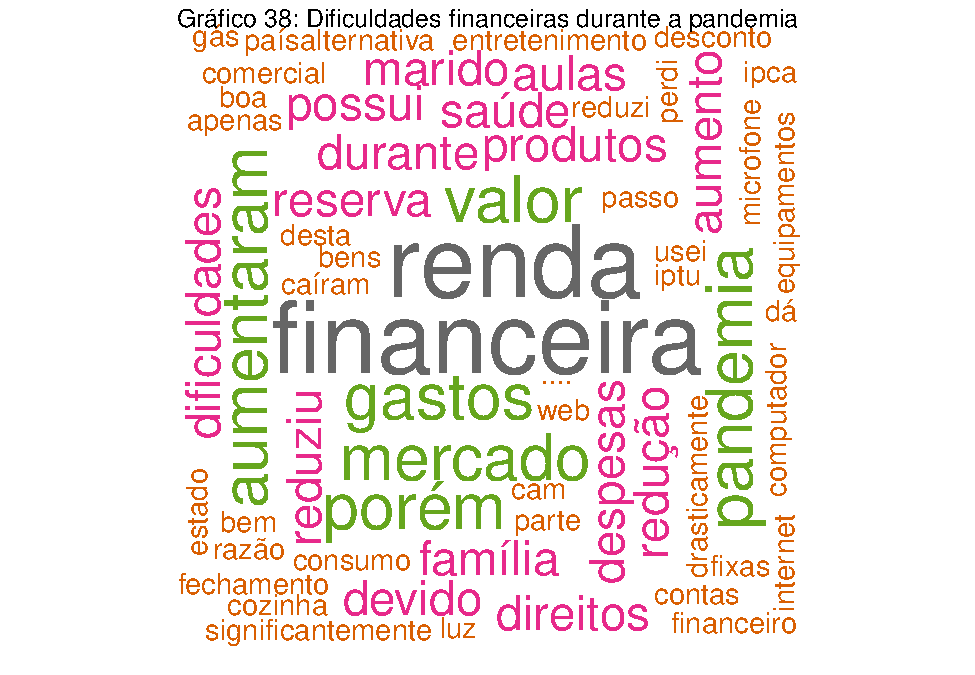
\includegraphics{consequencias-oriundas-da-pandemia-v1.0_files/figure-latex/grafico-38-1.pdf}

\begin{verbatim}
## [1] "Principais ocorrências de palavras das dificuldades financeiras durante a pandemia"
\end{verbatim}

\begin{verbatim}
## [1] "financeira = 5"
## [1] "renda = 5"
## [1] "aumentaram = 3"
## [1] "gastos = 3"
## [1] "pandemia = 3"
## [1] "mercado = 3"
## [1] "valor = 3"
## [1] "porém = 3"
\end{verbatim}

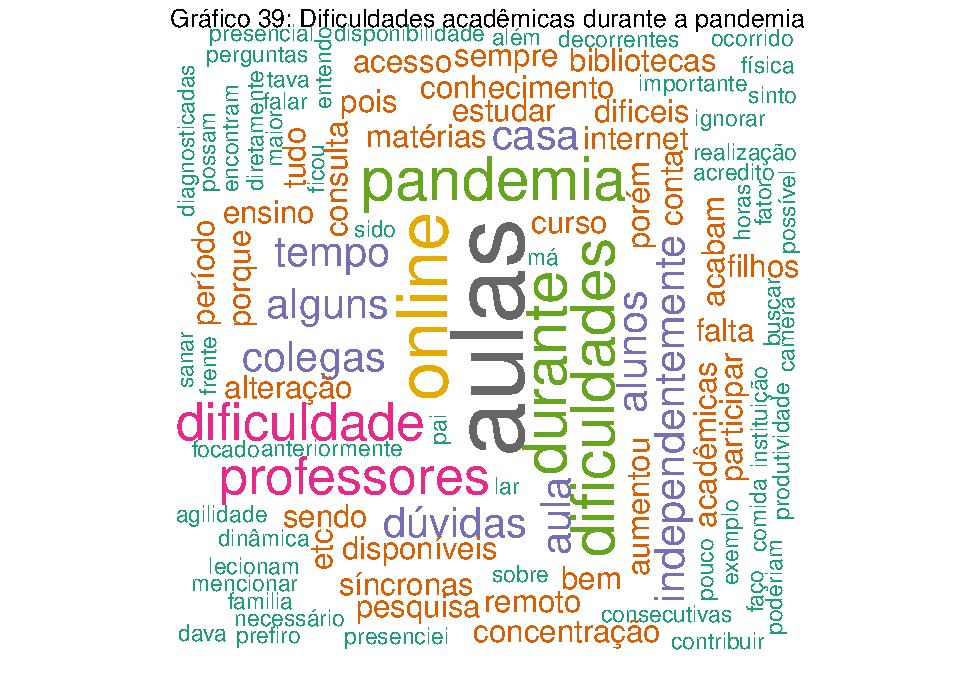
\includegraphics{consequencias-oriundas-da-pandemia-v1.0_files/figure-latex/grafico-sobrou-1.pdf}

\begin{verbatim}
## [1] "Principais ocorrências de palavras das dificuldades acadêmicas durante a pandemia"
\end{verbatim}

\begin{verbatim}
## [1] "aulas = 9"
## [1] "online = 6"
## [1] "durante = 5"
## [1] "dificuldades = 5"
## [1] "pandemia = 5"
## [1] "professores = 4"
## [1] "dificuldade = 4"
## [1] "tempo = 3"
## [1] "alguns = 3"
## [1] "alunos = 3"
## [1] "colegas = 3"
## [1] "dúvidas = 3"
## [1] "independentemente = 3"
## [1] "aula = 3"
## [1] "casa = 3"
\end{verbatim}

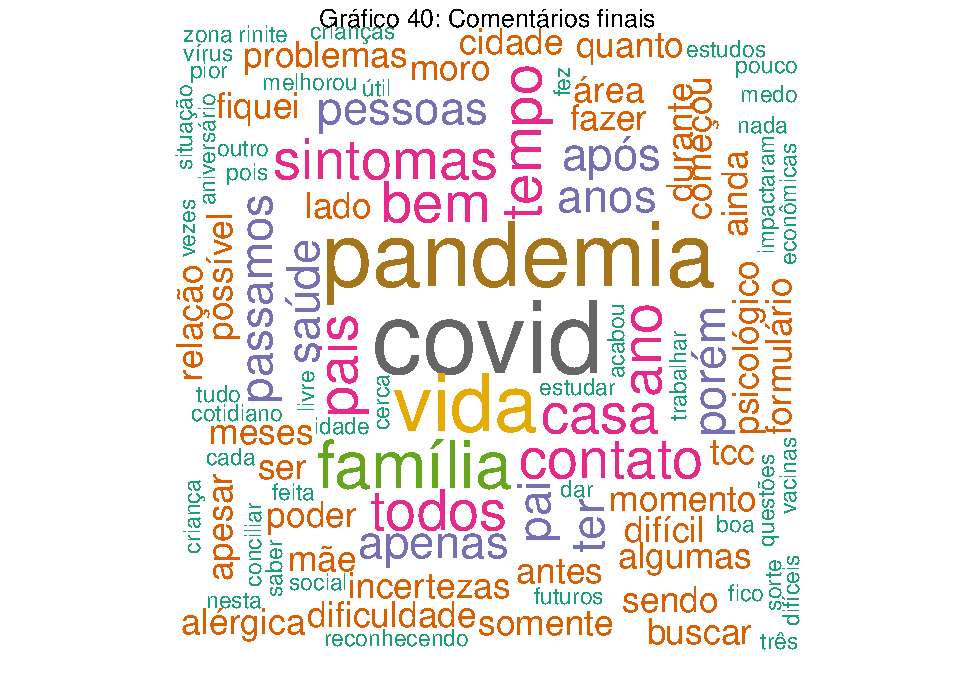
\includegraphics{consequencias-oriundas-da-pandemia-v1.0_files/figure-latex/grafico-40-1.pdf}

\begin{verbatim}
## [1] "Principais ocorrências de palavras nos comentários finais"
\end{verbatim}

\begin{verbatim}
## [1] "covid = 8"
## [1] "pandemia = 7"
## [1] "vida = 6"
## [1] "família = 5"
## [1] "casa = 4"
## [1] "tempo = 4"
## [1] "bem = 4"
## [1] "pais = 4"
## [1] "todos = 4"
## [1] "ano = 4"
## [1] "contato = 4"
## [1] "sintomas = 4"
## [1] "saúde = 3"
## [1] "anos = 3"
## [1] "pai = 3"
## [1] "passamos = 3"
## [1] "porém = 3"
## [1] "ter = 3"
## [1] "apenas = 3"
## [1] "pessoas = 3"
## [1] "após = 3"
\end{verbatim}

\hypertarget{sobras}{%
\subsection{Sobras ?}\label{sobras}}

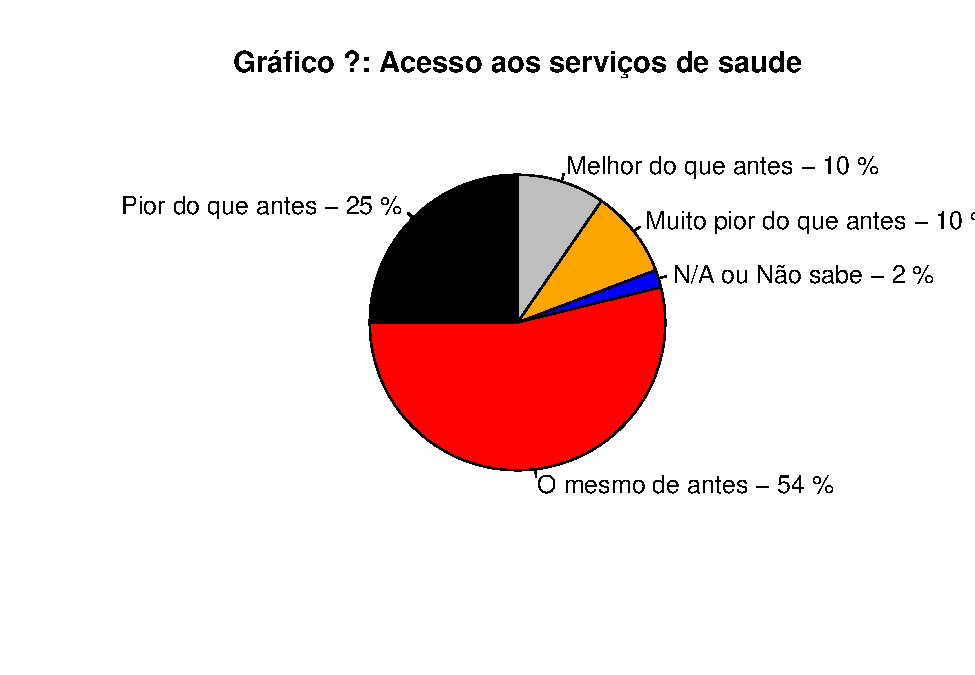
\includegraphics{consequencias-oriundas-da-pandemia-v1.0_files/figure-latex/grafico-nana-1.pdf}

\hypertarget{resultados-e-discussuxe3o}{%
\subsection{Resultados e Discussão}\label{resultados-e-discussuxe3o}}

Após a análise dos dados oriundos do questionário, foi observado que as
respostas recebidas não estão totalmente distantes da realidade
brasileira após período crítico de pandemia. Porém, deve-se ressaltar
alguns tópicos que chamam a atenção por revelarem informações sobre
dificuldades que, até então, pareciam representar uma parcela distante
da população comparada à bolha social de cada indivíduo.\\
Como primeiro exemplo, deve-se citar os 2\% universitários que não
migraram para o ensino virtual. Esse valor ainda foi superior que o
identificado em escolas públicas e particulares, segundo pesquisa
divulgada pela Agência Senado:

No ensino privado, 70,9\% das escolas ficaram fechadas no ano passado. O
número é consideravelmente menor que o da rede pública: 98,4\% das
escolas federais, 97,5\% das municipais e 85,9\% das estaduais. (Agência
Senado)

Contudo, de acordo com o Presidente da Comissão de Educação da Alerj
durante a pandemia, Flavio Serafini (Psol), a rede estadual não
conseguia apresentar (na época) uma solução que garantisse o direito ao
ensino durante a pandemia. Mais de um terço dos alunos sequer acessou o
aplicativo do estado, e a média de uso diário é inferior a 10\% do total
de estudantes na maioria dos dias. Isso mostra que o que foi
desenvolvido até agora é muito limitado. Faltou uma política de inclusão
digital mais estruturante.'' (EXTRA, 2021). Isso fez com que a qualidade
da aprendizagem caísse e o déficit educacional aumentasse, agravando
ainda mais a desigualdade. A crise financeira iniciada em 2014 foi
causada por um conjunto de choques de oferta e demanda, obrigando
gestores públicos a adotarem instrumentos políticos para atenuar seus
efeitos (Mariano, 2016), porém a tão temida crise da pandemia não teve
quaisquer indícios ou sinais semelhantes ao anterior. De acordo com o
relatório do Banco Mundial, a recessão decorrente da pandemia atingiu
seu ápice, em número de países atingidos, nos últimos 120 anos (PODER
360, 2022).

``O Brasil desembolsou 15\% do PIC (\ldots) para conter os efeitos da
covid no 1 ano de pandemia. (\ldots) O endividamento dos países tende a
se agravar, disse Ramalho, por outra consequência global da pandemia: a
alta da inflação.'' (PODER 360, 2022).

De acordo com a fonte, o Banco Mundial ainda estima que 76 milhões de
pessoas entraram em 2020 para a extrema pobreza. O crescimento da
desigualdade não foi causado apenas por conta da pandemia, contudo os
mais vulneráveis ficaram excluídos até de medidas como o Auxílio
Emergencial, já que muitos não têm acesso à internet. Segundo o IBGE, em
2021, 92,3\% dos domicílios urbanos brasileiros têm acesso à Internet
(PNAD, 2022). Entretanto, a desigualdade também se apresenta nesses
casos, já que 100\% dos lares da classe A têm ao menos um computador, e
apenas 13\% dos de classe D e E.\\
Paralelamente, é importante destacar que boa parte dos entrevistados
sofreram consequências mais brandas no âmbito educacional. Apesar de
enfrentarem as mesmas dificuldades, como por exemplo, a falta de acesso
à estrutura universitária em determinadas situações, de modo geral
pode-se concluir que não sofreram impactos grandiosos que resultam no
rompimento das atividades acadêmicas ou sua conclusão.

\hypertarget{conclusuxe3o}{%
\subsection{Conclusão}\label{conclusuxe3o}}

Diante dos resultados apresentados, conclui-se que a maior parte dos
estudantes universitários desta pesquisa conseguiu passar pelo período
problemático da pandemia sem grandes mudanças na sua vida acadêmica.\\
As universidades em que estão matriculados migraram para o ensino remoto
e adaptando-se às necessidades para atender os docentes, inclusive no
quesito infraestrutura, mesmo boa parte relatando algumas dificuldades
em acessá-la sem grandes problemas. No quesito financeiro, ao contrário
das expectativas de refletir o cenário nacional, os resultados mostraram
que boa parte não sofreu grandes impactos e puderam continuar com sua
rotina sem alardes. Um ponto interessante a ser citado uma vez que,
mesmo possuindo fonte de renda, alguns receberam auxílio para
complementar.\\
Quanto ao desempenho durante o período de ensino remoto, ainda que
alguns sentiram maiores dificuldades e até mesmo uma queda em sua
performance, conta-se um desempenho positivo entre a maioria que manteve
a mesma produtividade.\\
Uma das principais limitações deste estudo é o fato de a amostra engloba
basicamente estudantes de uma única universidade pública no Brasil, ou
seja, os resultados podem não ser representativos de toda a população
universitária em nível nacional ou até mesmo regional. No entanto, a
taxa está dentro da faixa esperada de respostas pelos autores, usando
pesquisas on-line com estudantes universitários.\\
Considerando que não usamos uma amostragem aleatória e que a prevalência
de problemas financeiros, logísticos de isolamento, de desempenho
estudantil, e satisfação quanto às medidas adotadas pelas universidades,
podem variar de acordo com o momento em que a avaliação foi feita, e
concepção pessoal. Por conta das diferenças populacionais, e
instrumentos usados, comparações entre outros levantamentos e pesquisas
devem ser feitas com cautela.

\hypertarget{bibliografia}{%
\subsection{Bibliografia}\label{bibliografia}}

BUTANTAN. Por que acontecem mutações do SARS-CoV-2 e quais as diferenças
entre cada uma das variantes. 2021 . Disponível em:
\url{https://butantan.gov.br/noticias/por-que-acontecem-mutacoes-do-sars-cov-2-e-quais-as-diferencas-entre-cada-uma-das-variantes}.

BRICEÑO-LEÓN, R. (2003). Quatro modelos de integração de técnicas
qualitativas e quantitativas de investigação nas ciências sociais. O
Clássico e o novo--tendências, objetos e abordagens em ciências sociais
e saúde, 157-186. Disponível em:
\url{https://books.scielo.org/id/d5t55/pdf/goldenberg-9788575412510.pdf\#page=157}.

CAMPOS, Mônica Rodrigues et al.~Carga de doença da COVID-19 e de suas
complicações agudas e crônicas: reflexões sobre a mensuração (DALY) e
perspectivas no Sistema Único de Saúde. Cadernos de Saúde Pública
{[}online{]}. v. 36, n.~11. Disponível em:
\url{https://doi.org/10.1590/0102-311X00148920}. ISSN 1678-4464.
\url{https://doi.org/10.1590/0102-311X00148920}. Acessado 23 Janeiro
2023.

CEPAL. Pandemia provoca aumento nos níveis de pobreza sem precedentes
nas últimas décadas e tem um forte impacto na desigualdade e no emprego.
2021. Disponível em:
\url{https://www.cepal.org/pt-br/comunicados/pandemia-provoca-aumento-niveis-pobreza-sem-precedentes-ultimas-decadas-tem-forte}.

DE NEGRI, Fernanda et al.~Ciência e Tecnologia frente à pandemia: Como a
pesquisa científica e a inovação estão ajudando a combater o novo
coronavírus no Brasil e no mundo. Centro de Pesquisa em Ciência,
Tecnologia e Sociedade. IPEA, Brasília, DF. 23 dez. 2020. Disponível em:
\url{https://www.ipea.gov.br/cts/pt/central-de-conteudo/artigos/artigos/182-corona}.
Acesso em: 14 mai. 2022.

EXTRA. Migração para as escolas públicas cresce 30\% na pandemia, e rede
privada perde 50 mil alunos. 2021. Disponível em:
\url{https://extra.globo.com/noticias/rio/migracao-para-as-escolas-publicas-cresce-30-na-pandemia-rede-privada-perde-50-mil-alunos-25138212.html}.

FIOCRUZ. 2021. Aula inaugural analisa consequências das decisões
brasileiras no enfrentamento à pandemia. Disponível em:
\url{https://informe.ensp.fiocruz.br/noticias/51262}.

GUSSO, Hélder Lima et al.~Ensino Superior em Tempos de Pandemia:
Diretrizes à Gestão Universitária. Educação \& Sociedade, vol.~41,
p.~1-27, set. 2020.

IBGE. PNAD Contínua - Módulo de Tecnologia de Informação e Comunicação
(TIC) 2021. Disponível em:
\url{https://www.ibge.gov.br/estatisticas/multidominio/ciencia-tecnologia-e-inovacao/17270-pnad-continua.html?=\&t=resultados}.

JAMES, G., WITTEN, D., HASTIE, T., TIBSHIRANI, R. (2013). An
Introduction to Statistical Learning. Springer.

MARIANO, Jefferson, Barcellos, Lívia I. (2017). Estratégias de gestão
dos municípios em cenário de crise socioeconômica. Geografia e Pesquisa,
11(2).

MORAES, Rodrigo Fracalossi de. Medidas Legais de Incentivo ao
Distanciamento Social: Comparação das Políticas de Governos Estaduais e
Prefeituras das Capitais no Brasil. IPEA, Brasília, DF, abr. 2020.
Disponível em: \url{http://}
\url{https://repositorio.ipea.gov.br/handle/11058/10096}. Acesso em: 13
mar. 2023.

O GLOBO. Por que o negacionismo atrapalha o combate à Covid?. 2021.
Disponível em:
\url{https://oglobo.globo.com/podcast/por-que-negacionismo-atrapalha-combate-covid-1-24931788}.

PODER 360. Pandemia causou recessão mais ampla que as guerras mundiais.
2022. Disponível em:
\url{https://www.poder360.com.br/economia/pandemia-causou-recessao-mais-ampla-que-as-guerras-mundiais/}.

UOL. Covid: 172,6 milhões de brasileiros completam vacinação, 80,3\% da
população. Disponível em:
\url{https://noticias.uol.com.br/saude/ultimas-noticias/redacao/2023/01/11/vacinacao-covid-19-coronavirus-11-de-janeiro.htm?cmpid=copiaecola}.
Acesso em: 12 de jan. de 2023.

UNA-SUS. Organização Mundial de Saúde declara pandemia do novo
Coronavírus. Disponível em:
\url{https://www.unasus.gov.br/noticia/organizacao-mundial-de-saude-declara-pandemia-de-coronavirus}.
Acesso em: 10 de jan. de 2023.

VEJA. As lições da pandemia de Covid-19 -- que está chegando ao fim.
2021 . Disponível em:
\url{https://veja.abril.com.br/saude/os-sinais-de-que-a-pandemia-de-covid-19-vai-acabar-em-breve/}.

World Health Organization. (2020). Pandemic influenza preparedness and
response: A WHO guidance document. Disponível em:
\url{https://www.who.int/csr/disease/influenza/pipguidance2009/en/}.
Acesso em 13 mar. 2023.

\end{document}
